%!TEX program = xelatex
\PassOptionsToPackage{table,svgnames}{xcolor}
\PassOptionsToPackage{english}{translator}
\documentclass[aspectratio=169,11pt]{beamer}

%----------------------------------------
% Packages
%----------------------------------------
%\usepackage[utf8]{inputenc}
\usepackage[T1]{fontenc}
\usepackage[english]{babel} % Second language = main language
\usepackage{translator}
\usepackage{lmodern}
\usepackage{hyperref}
\usepackage{xcolor}
\usepackage{listings}
\usepackage{amsmath}
\usepackage{amssymb}
\usepackage{mathrsfs}
\usepackage{array}
\usepackage{tabularx}
\usepackage{multirow}
\usepackage[justification=centering]{caption}
\usepackage[nomessages]{fp}
\usepackage{float}
\usepackage{standalone}
\usepackage{import}
% PGF-TikZ
\usepackage{pgf}
\usepackage{tikz}
\usepackage{pgf-umlsd}
\usepackage{pgfgantt}

%----------------------------------------
% Theme
%----------------------------------------

% \usetheme{boxes}
% \useoutertheme{infolines}
% \usecolortheme{whale}%beaver
% \usecolortheme{seagull}

\usetheme[illustration=cover]{utbm}
%\usetheme{utbm}

% remove bottom line
%\setbeamertemplate{footline}{}

% remove navigation symbols.
\beamertemplatenavigationsymbolsempty{}

%\setbeamercovered{transparent}

%----------------------------------------
% Informations
%----------------------------------------

\title{Generation of the hyperplanes of  \texorpdfstring{$S_k(3)$}{S\_k(3)} }
\subtitle{TX52}
\author{Jérôme Boulmier, Maxime Pinard}
\institute[UTBM]{Université de Technologie de Belfort Montbéliard}
\date[2018-06-29]{29 June 2018}

%\keywords{}
\subject{TX52, Generation of the geometric hyperplanes of  \texorpdfstring{$S_k(3)$}{S\_k(3)}}
%\logo{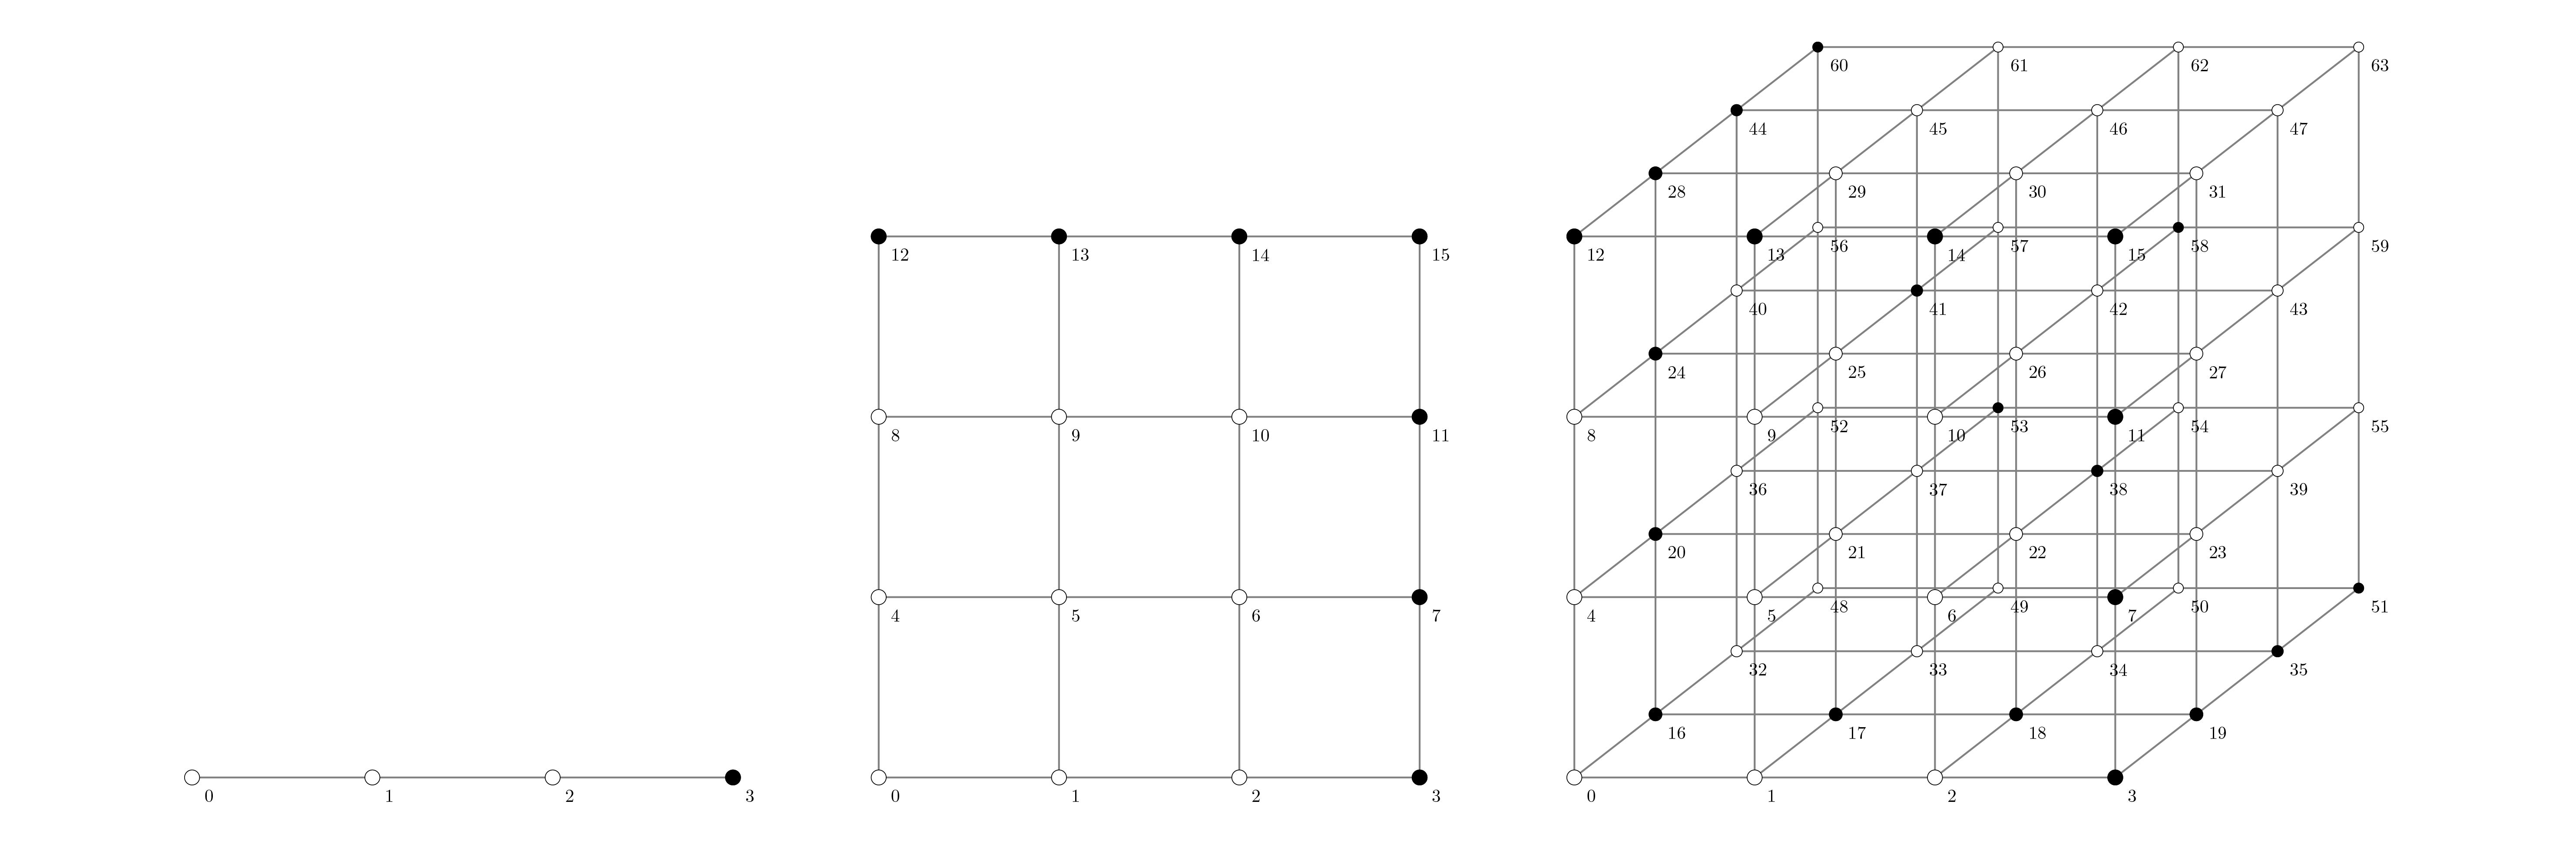
\includegraphics[width=0.12\textwidth]{cover}}

%----------------------------------------
% Configurations
%----------------------------------------

\graphicspath{{figures/}}

% \AtBeginSection
% {
% 	\begin{frame}<beamer>
% 		\vfill{}
% 		\centering
% 		\begin{beamercolorbox}[sep=8pt,center]{title}
% 			\Huge\insertsectionhead\par%
% 		\end{beamercolorbox}
% 		\vfill{}
% 	\end{frame}
% }

\AtBeginSection
{
	\begin{frame}[plain]
		\utbmtitle{\insertsectionhead}
	\end{frame}
}

\makeatletter
\let\@@magyar@captionfix\relax
\makeatother

%----------------------------------------
% Figures configuration
%----------------------------------------

\usetikzlibrary{shapes.geometric}
\usetikzlibrary{arrows.meta}
\usetikzlibrary{calc}
\usetikzlibrary{matrix}
\usetikzlibrary{fit}

\pgfmathsetmacro\pointsPerLine{4}

%---------------------------------
% Colors
\colorlet{points_boder_color}{black}%
\colorlet{points_color}{white}%
\colorlet{in_points_color}{black}%
\colorlet{lines_color}{gray}%

%---------------------------------
% Sizes
\pgfmathsetmacro\pointssep{100}%
\pgfmathsetmacro\pointssize{10}%
\pgfmathsetmacro\lineswidth{1}%

\newcommand{\inPoints}{}

%----------------------------------------
% Document
%----------------------------------------
\begin{document}
	\begin{frame}[plain,noframenumbering]
		\titlepage
	\end{frame}
	% \begin{frame}{Table of contents}
	% 	\tableofcontents
	% \end{frame}
	%!TEX root = ./main.tex

\newsavebox\truehyperplane
\sbox{\truehyperplane}{%
	\pgfmathsetmacro\dimension{2}% in [0,3]
	\renewcommand{\inPoints}{0,1,2,3,4,8,12}%
	%---------------------------------
% Auto config
\pgfmathsetmacro\xdim{\dimension>0}%
\pgfmathsetmacro\ydim{\dimension>1}%
\pgfmathsetmacro\zdim{\dimension>2}%
\pgfmathsetmacro\pointsPerLineMinusOne{\pointsPerLine-1}%
\pgfmathsetmacro\xnbr{\pointsPerLineMinusOne*\xdim}%
\pgfmathsetmacro\ynbr{\pointsPerLineMinusOne*\ydim}%
\pgfmathsetmacro\znbr{\pointsPerLineMinusOne*\zdim}%

%---------------------------------
% Figure
\begin{tikzpicture}[x={(1pt,0pt)},y={(0pt,1pt)},z={(0.45pt,0.35pt)}]
	\tikzset{point/.style={
		draw,
		circle,
		minimum size=\pointsize,
		inner sep=0,
	}}

	% Coordinates
	\foreach \x in {0,...,\xnbr}
	{
		\foreach \y in {0,...,\ynbr}
		{
			\foreach \z in {0,...,\znbr}
			{
				\pgfmathsetmacro\num{int(\x+(\pointsPerLine*\y)+(\pointsPerLine*\pointsPerLine*\z))}
				\coordinate (point\num) at (\pointssep*\x,\pointssep*\y,\pointssep*\z) {};
				\coordinate (point_\x_\y_\z) at (\pointssep*\x,\pointssep*\y,\pointssep*\z) {};
			}
		}
	}

	% Lines
	\foreach \x in {0,...,\xnbr}
	{
		\foreach \y in {0,...,\ynbr}
		{
			\foreach \z in {0,...,\znbr}
			{
				\ifthenelse{\x=0}{}{
					\pgfmathsetmacro\lastx{int(\x-1)}
					\draw[line width=\lineswidth,lines_color] (point_\lastx_\y_\z) -- (point_\x_\y_\z);
				}
				\ifthenelse{\y=0}{}{
					\pgfmathsetmacro\lasty{int(\y-1)}
					\draw[line width=\lineswidth,lines_color] (point_\x_\lasty_\z) -- (point_\x_\y_\z);
				}
				\ifthenelse{\z=0}{}{
					\pgfmathsetmacro\lastz{int(\z-1)}
					\draw[line width=\lineswidth,lines_color] (point_\x_\y_\lastz) -- (point_\x_\y_\z);
				}
			}
		}
	}

	% Points and numbers
	\foreach \x in {0,...,\xnbr}
	{
		\foreach \y in {0,...,\ynbr}
		{
			\foreach \z in {0,...,\znbr}
			{
				% Config
				\pgfmathsetmacro\num{int(\x+(\pointsPerLine*\y)+(\pointsPerLine*\pointsPerLine*\z))}
				\pgfmathsetmacro\pointsize{\pointssize*5/(5+\z+1)}

				% Draw point
				\node[
					point,
					points_boder_color,
					fill=points_color
				] at (point_\x_\y_\z.center) {};

				% Fill point if is in
				\foreach \i in \inPoints
				{
					\ifthenelse{\num=\i}{
						\node[
							point,
							points_boder_color,
							fill=in_points_color
						] at (point\i.center) {};
					}{}
				}

				% Number
				\pgfmathsetmacro\num{int(\x+(\pointsPerLine*\y)+(\pointsPerLine*\pointsPerLine*\z))}
				\node[below right=3pt] at (point_\x_\y_\z.center) {\small\num};
			}
		}
	}
\end{tikzpicture}
%
}

\begin{frame}
	\frametitle{Definition}
	\begin{block}{Geometric hyperplane}
		An hyperplane $H$ is a proper subspace of $S_k(3)$ such that for each line of $S_k(3)$, $H$ either contain the full line or only one point of the line.
	\end{block}
	\centering%
	\resizebox{0.7\textwidth}{!}{
		\begin{tikzpicture}
			\node (falsehyperplane) at (0,0) {%!TEX root = ../main.tex

\pgfmathsetmacro\dimension{2}% in [0,3]
\renewcommand{\inPoints}{1,2,4,9,15}%

%---------------------------------
% Auto config
\pgfmathsetmacro\xdim{\dimension>0}%
\pgfmathsetmacro\ydim{\dimension>1}%
\pgfmathsetmacro\zdim{\dimension>2}%
\pgfmathsetmacro\pointsPerLineMinusOne{\pointsPerLine-1}%
\pgfmathsetmacro\xnbr{\pointsPerLineMinusOne*\xdim}%
\pgfmathsetmacro\ynbr{\pointsPerLineMinusOne*\ydim}%
\pgfmathsetmacro\znbr{\pointsPerLineMinusOne*\zdim}%

%---------------------------------
% Figure
\begin{tikzpicture}[x={(1pt,0pt)},y={(0pt,1pt)},z={(0.45pt,0.35pt)}]
	\tikzset{point/.style={
		draw,
		circle,
		minimum size=\pointsize,
		inner sep=0,
	}}

	% Coordinates
	\foreach \x in {0,...,\xnbr}
	{
		\foreach \y in {0,...,\ynbr}
		{
			\foreach \z in {0,...,\znbr}
			{
				\pgfmathsetmacro\num{int(\x+(\pointsPerLine*\y)+(\pointsPerLine*\pointsPerLine*\z))}
				\coordinate (point\num) at (\pointssep*\x,\pointssep*\y,\pointssep*\z) {};
				\coordinate (point_\x_\y_\z) at (\pointssep*\x,\pointssep*\y,\pointssep*\z) {};
			}
		}
	}

	\uncover<2->{

		% Lines
		\foreach \x in {0,...,\xnbr}
		{
			\foreach \y in {0,...,\ynbr}
			{
				\foreach \z in {0,...,\znbr}
				{
					\ifthenelse{\x=0}{}{
						\pgfmathsetmacro\lastx{int(\x-1)}
						\draw[line width=\lineswidth,lines_color] (point_\lastx_\y_\z) -- (point_\x_\y_\z);
					}
					\ifthenelse{\y=0}{}{
						\pgfmathsetmacro\lasty{int(\y-1)}
						\draw[line width=\lineswidth,lines_color] (point_\x_\lasty_\z) -- (point_\x_\y_\z);
					}
					\ifthenelse{\z=0}{}{
						\pgfmathsetmacro\lastz{int(\z-1)}
						\draw[line width=\lineswidth,lines_color] (point_\x_\y_\lastz) -- (point_\x_\y_\z);
					}
				}
			}
		}

		% Points and numbers
		\foreach \x in {0,...,\xnbr}
		{
			\foreach \y in {0,...,\ynbr}
			{
				\foreach \z in {0,...,\znbr}
				{
					% Config
					\pgfmathsetmacro\num{int(\x+(\pointsPerLine*\y)+(\pointsPerLine*\pointsPerLine*\z))}
					\pgfmathsetmacro\pointsize{\pointssize*5/(5+\z+1)}

					% Draw point
					\node[
						point,
						points_boder_color,
						fill=points_color
					] at (point_\x_\y_\z.center) {};

					% Fill point if is in
					\foreach \i in \inPoints
					{
						\ifthenelse{\num=\i}{
							\node[
								point,
								points_boder_color,
								fill=in_points_color
							] at (point\i.center) {};
						}{}
					}

					% Number
					\pgfmathsetmacro\num{int(\x+(\pointsPerLine*\y)+(\pointsPerLine*\pointsPerLine*\z))}
					\node[below right=3pt] at (point_\x_\y_\z.center) {\small\num};
				}
			}
		}

	}

	\uncover<3->{
		\node[fit=(point_1_0_0)(point_2_0_0), draw, ultra thick, red, ellipse, minimum height=20] {};
	}
	\uncover<4->{
		\draw[ultra thick, red] (point_0_0_0.center) -- (point_3_3_0.center);
		\draw[ultra thick, red] (point_3_0_0.center) -- (point_0_3_0.center);
	}
\end{tikzpicture}
};
			\uncover<2->{
				\node[anchor=south west, xshift=50] (truehyperplane) at (falsehyperplane.south east) {\usebox{\truehyperplane}};
			}
		\end{tikzpicture}
	}
\end{frame}

	%!TEX root = ./main.tex

%---------------------------------
% Geometry
\pgfmathsetmacro\dimension{2}% in [0,3]
\pgfmathsetmacro\pointsPerLine{4}% in [1,\infty[

\begin{frame}
	\frametitle{Dimension 2 hyperplanes}
	\renewcommand{\inPoints}{3,6,9,12}%
	\resizebox{0.09\textwidth}{!}{%---------------------------------
% Auto config
\pgfmathsetmacro\xdim{\dimension>0}%
\pgfmathsetmacro\ydim{\dimension>1}%
\pgfmathsetmacro\zdim{\dimension>2}%
\pgfmathsetmacro\pointsPerLineMinusOne{\pointsPerLine-1}%
\pgfmathsetmacro\xnbr{\pointsPerLineMinusOne*\xdim}%
\pgfmathsetmacro\ynbr{\pointsPerLineMinusOne*\ydim}%
\pgfmathsetmacro\znbr{\pointsPerLineMinusOne*\zdim}%

%---------------------------------
% Figure
\begin{tikzpicture}[x={(1pt,0pt)},y={(0pt,1pt)},z={(0.45pt,0.35pt)}]
	\tikzset{point/.style={
		draw,
		circle,
		minimum size=\pointsize,
		inner sep=0,
	}}

	% Coordinates
	\foreach \x in {0,...,\xnbr}
	{
		\foreach \y in {0,...,\ynbr}
		{
			\foreach \z in {0,...,\znbr}
			{
				\pgfmathsetmacro\num{int(\x+(\pointsPerLine*\y)+(\pointsPerLine*\pointsPerLine*\z))}
				\coordinate (point\num) at (\pointssep*\x,\pointssep*\y,\pointssep*\z) {};
				\coordinate (point_\x_\y_\z) at (\pointssep*\x,\pointssep*\y,\pointssep*\z) {};
			}
		}
	}

	% Lines
	\foreach \x in {0,...,\xnbr}
	{
		\foreach \y in {0,...,\ynbr}
		{
			\foreach \z in {0,...,\znbr}
			{
				\ifthenelse{\x=0}{}{
					\pgfmathsetmacro\lastx{int(\x-1)}
					\draw[line width=\lineswidth,lines_color] (point_\lastx_\y_\z) -- (point_\x_\y_\z);
				}
				\ifthenelse{\y=0}{}{
					\pgfmathsetmacro\lasty{int(\y-1)}
					\draw[line width=\lineswidth,lines_color] (point_\x_\lasty_\z) -- (point_\x_\y_\z);
				}
				\ifthenelse{\z=0}{}{
					\pgfmathsetmacro\lastz{int(\z-1)}
					\draw[line width=\lineswidth,lines_color] (point_\x_\y_\lastz) -- (point_\x_\y_\z);
				}
			}
		}
	}

	% Points and numbers
	\foreach \x in {0,...,\xnbr}
	{
		\foreach \y in {0,...,\ynbr}
		{
			\foreach \z in {0,...,\znbr}
			{
				% Config
				\pgfmathsetmacro\num{int(\x+(\pointsPerLine*\y)+(\pointsPerLine*\pointsPerLine*\z))}
				\pgfmathsetmacro\pointsize{\pointssize*5/(5+\z+1)}

				% Draw point
				\node[
					point,
					points_boder_color,
					fill=points_color
				] at (point_\x_\y_\z.center) {};

				% Fill point if is in
				\foreach \i in \inPoints
				{
					\ifthenelse{\num=\i}{
						\node[
							point,
							points_boder_color,
							fill=in_points_color
						] at (point\i.center) {};
					}{}
				}

				% Number
				\pgfmathsetmacro\num{int(\x+(\pointsPerLine*\y)+(\pointsPerLine*\pointsPerLine*\z))}
				\node[below right=3pt] at (point_\x_\y_\z.center) {\small\num};
			}
		}
	}
\end{tikzpicture}
}
	\renewcommand{\inPoints}{2,7,9,12}%
	\resizebox{0.09\textwidth}{!}{%---------------------------------
% Auto config
\pgfmathsetmacro\xdim{\dimension>0}%
\pgfmathsetmacro\ydim{\dimension>1}%
\pgfmathsetmacro\zdim{\dimension>2}%
\pgfmathsetmacro\pointsPerLineMinusOne{\pointsPerLine-1}%
\pgfmathsetmacro\xnbr{\pointsPerLineMinusOne*\xdim}%
\pgfmathsetmacro\ynbr{\pointsPerLineMinusOne*\ydim}%
\pgfmathsetmacro\znbr{\pointsPerLineMinusOne*\zdim}%

%---------------------------------
% Figure
\begin{tikzpicture}[x={(1pt,0pt)},y={(0pt,1pt)},z={(0.45pt,0.35pt)}]
	\tikzset{point/.style={
		draw,
		circle,
		minimum size=\pointsize,
		inner sep=0,
	}}

	% Coordinates
	\foreach \x in {0,...,\xnbr}
	{
		\foreach \y in {0,...,\ynbr}
		{
			\foreach \z in {0,...,\znbr}
			{
				\pgfmathsetmacro\num{int(\x+(\pointsPerLine*\y)+(\pointsPerLine*\pointsPerLine*\z))}
				\coordinate (point\num) at (\pointssep*\x,\pointssep*\y,\pointssep*\z) {};
				\coordinate (point_\x_\y_\z) at (\pointssep*\x,\pointssep*\y,\pointssep*\z) {};
			}
		}
	}

	% Lines
	\foreach \x in {0,...,\xnbr}
	{
		\foreach \y in {0,...,\ynbr}
		{
			\foreach \z in {0,...,\znbr}
			{
				\ifthenelse{\x=0}{}{
					\pgfmathsetmacro\lastx{int(\x-1)}
					\draw[line width=\lineswidth,lines_color] (point_\lastx_\y_\z) -- (point_\x_\y_\z);
				}
				\ifthenelse{\y=0}{}{
					\pgfmathsetmacro\lasty{int(\y-1)}
					\draw[line width=\lineswidth,lines_color] (point_\x_\lasty_\z) -- (point_\x_\y_\z);
				}
				\ifthenelse{\z=0}{}{
					\pgfmathsetmacro\lastz{int(\z-1)}
					\draw[line width=\lineswidth,lines_color] (point_\x_\y_\lastz) -- (point_\x_\y_\z);
				}
			}
		}
	}

	% Points and numbers
	\foreach \x in {0,...,\xnbr}
	{
		\foreach \y in {0,...,\ynbr}
		{
			\foreach \z in {0,...,\znbr}
			{
				% Config
				\pgfmathsetmacro\num{int(\x+(\pointsPerLine*\y)+(\pointsPerLine*\pointsPerLine*\z))}
				\pgfmathsetmacro\pointsize{\pointssize*5/(5+\z+1)}

				% Draw point
				\node[
					point,
					points_boder_color,
					fill=points_color
				] at (point_\x_\y_\z.center) {};

				% Fill point if is in
				\foreach \i in \inPoints
				{
					\ifthenelse{\num=\i}{
						\node[
							point,
							points_boder_color,
							fill=in_points_color
						] at (point\i.center) {};
					}{}
				}

				% Number
				\pgfmathsetmacro\num{int(\x+(\pointsPerLine*\y)+(\pointsPerLine*\pointsPerLine*\z))}
				\node[below right=3pt] at (point_\x_\y_\z.center) {\small\num};
			}
		}
	}
\end{tikzpicture}
}
	\renewcommand{\inPoints}{3,5,10,12}%
	\resizebox{0.09\textwidth}{!}{%---------------------------------
% Auto config
\pgfmathsetmacro\xdim{\dimension>0}%
\pgfmathsetmacro\ydim{\dimension>1}%
\pgfmathsetmacro\zdim{\dimension>2}%
\pgfmathsetmacro\pointsPerLineMinusOne{\pointsPerLine-1}%
\pgfmathsetmacro\xnbr{\pointsPerLineMinusOne*\xdim}%
\pgfmathsetmacro\ynbr{\pointsPerLineMinusOne*\ydim}%
\pgfmathsetmacro\znbr{\pointsPerLineMinusOne*\zdim}%

%---------------------------------
% Figure
\begin{tikzpicture}[x={(1pt,0pt)},y={(0pt,1pt)},z={(0.45pt,0.35pt)}]
	\tikzset{point/.style={
		draw,
		circle,
		minimum size=\pointsize,
		inner sep=0,
	}}

	% Coordinates
	\foreach \x in {0,...,\xnbr}
	{
		\foreach \y in {0,...,\ynbr}
		{
			\foreach \z in {0,...,\znbr}
			{
				\pgfmathsetmacro\num{int(\x+(\pointsPerLine*\y)+(\pointsPerLine*\pointsPerLine*\z))}
				\coordinate (point\num) at (\pointssep*\x,\pointssep*\y,\pointssep*\z) {};
				\coordinate (point_\x_\y_\z) at (\pointssep*\x,\pointssep*\y,\pointssep*\z) {};
			}
		}
	}

	% Lines
	\foreach \x in {0,...,\xnbr}
	{
		\foreach \y in {0,...,\ynbr}
		{
			\foreach \z in {0,...,\znbr}
			{
				\ifthenelse{\x=0}{}{
					\pgfmathsetmacro\lastx{int(\x-1)}
					\draw[line width=\lineswidth,lines_color] (point_\lastx_\y_\z) -- (point_\x_\y_\z);
				}
				\ifthenelse{\y=0}{}{
					\pgfmathsetmacro\lasty{int(\y-1)}
					\draw[line width=\lineswidth,lines_color] (point_\x_\lasty_\z) -- (point_\x_\y_\z);
				}
				\ifthenelse{\z=0}{}{
					\pgfmathsetmacro\lastz{int(\z-1)}
					\draw[line width=\lineswidth,lines_color] (point_\x_\y_\lastz) -- (point_\x_\y_\z);
				}
			}
		}
	}

	% Points and numbers
	\foreach \x in {0,...,\xnbr}
	{
		\foreach \y in {0,...,\ynbr}
		{
			\foreach \z in {0,...,\znbr}
			{
				% Config
				\pgfmathsetmacro\num{int(\x+(\pointsPerLine*\y)+(\pointsPerLine*\pointsPerLine*\z))}
				\pgfmathsetmacro\pointsize{\pointssize*5/(5+\z+1)}

				% Draw point
				\node[
					point,
					points_boder_color,
					fill=points_color
				] at (point_\x_\y_\z.center) {};

				% Fill point if is in
				\foreach \i in \inPoints
				{
					\ifthenelse{\num=\i}{
						\node[
							point,
							points_boder_color,
							fill=in_points_color
						] at (point\i.center) {};
					}{}
				}

				% Number
				\pgfmathsetmacro\num{int(\x+(\pointsPerLine*\y)+(\pointsPerLine*\pointsPerLine*\z))}
				\node[below right=3pt] at (point_\x_\y_\z.center) {\small\num};
			}
		}
	}
\end{tikzpicture}
}
	\renewcommand{\inPoints}{1,7,10,12}%
	\resizebox{0.09\textwidth}{!}{%---------------------------------
% Auto config
\pgfmathsetmacro\xdim{\dimension>0}%
\pgfmathsetmacro\ydim{\dimension>1}%
\pgfmathsetmacro\zdim{\dimension>2}%
\pgfmathsetmacro\pointsPerLineMinusOne{\pointsPerLine-1}%
\pgfmathsetmacro\xnbr{\pointsPerLineMinusOne*\xdim}%
\pgfmathsetmacro\ynbr{\pointsPerLineMinusOne*\ydim}%
\pgfmathsetmacro\znbr{\pointsPerLineMinusOne*\zdim}%

%---------------------------------
% Figure
\begin{tikzpicture}[x={(1pt,0pt)},y={(0pt,1pt)},z={(0.45pt,0.35pt)}]
	\tikzset{point/.style={
		draw,
		circle,
		minimum size=\pointsize,
		inner sep=0,
	}}

	% Coordinates
	\foreach \x in {0,...,\xnbr}
	{
		\foreach \y in {0,...,\ynbr}
		{
			\foreach \z in {0,...,\znbr}
			{
				\pgfmathsetmacro\num{int(\x+(\pointsPerLine*\y)+(\pointsPerLine*\pointsPerLine*\z))}
				\coordinate (point\num) at (\pointssep*\x,\pointssep*\y,\pointssep*\z) {};
				\coordinate (point_\x_\y_\z) at (\pointssep*\x,\pointssep*\y,\pointssep*\z) {};
			}
		}
	}

	% Lines
	\foreach \x in {0,...,\xnbr}
	{
		\foreach \y in {0,...,\ynbr}
		{
			\foreach \z in {0,...,\znbr}
			{
				\ifthenelse{\x=0}{}{
					\pgfmathsetmacro\lastx{int(\x-1)}
					\draw[line width=\lineswidth,lines_color] (point_\lastx_\y_\z) -- (point_\x_\y_\z);
				}
				\ifthenelse{\y=0}{}{
					\pgfmathsetmacro\lasty{int(\y-1)}
					\draw[line width=\lineswidth,lines_color] (point_\x_\lasty_\z) -- (point_\x_\y_\z);
				}
				\ifthenelse{\z=0}{}{
					\pgfmathsetmacro\lastz{int(\z-1)}
					\draw[line width=\lineswidth,lines_color] (point_\x_\y_\lastz) -- (point_\x_\y_\z);
				}
			}
		}
	}

	% Points and numbers
	\foreach \x in {0,...,\xnbr}
	{
		\foreach \y in {0,...,\ynbr}
		{
			\foreach \z in {0,...,\znbr}
			{
				% Config
				\pgfmathsetmacro\num{int(\x+(\pointsPerLine*\y)+(\pointsPerLine*\pointsPerLine*\z))}
				\pgfmathsetmacro\pointsize{\pointssize*5/(5+\z+1)}

				% Draw point
				\node[
					point,
					points_boder_color,
					fill=points_color
				] at (point_\x_\y_\z.center) {};

				% Fill point if is in
				\foreach \i in \inPoints
				{
					\ifthenelse{\num=\i}{
						\node[
							point,
							points_boder_color,
							fill=in_points_color
						] at (point\i.center) {};
					}{}
				}

				% Number
				\pgfmathsetmacro\num{int(\x+(\pointsPerLine*\y)+(\pointsPerLine*\pointsPerLine*\z))}
				\node[below right=3pt] at (point_\x_\y_\z.center) {\small\num};
			}
		}
	}
\end{tikzpicture}
}
	\renewcommand{\inPoints}{2,5,11,12}%
	\resizebox{0.09\textwidth}{!}{%---------------------------------
% Auto config
\pgfmathsetmacro\xdim{\dimension>0}%
\pgfmathsetmacro\ydim{\dimension>1}%
\pgfmathsetmacro\zdim{\dimension>2}%
\pgfmathsetmacro\pointsPerLineMinusOne{\pointsPerLine-1}%
\pgfmathsetmacro\xnbr{\pointsPerLineMinusOne*\xdim}%
\pgfmathsetmacro\ynbr{\pointsPerLineMinusOne*\ydim}%
\pgfmathsetmacro\znbr{\pointsPerLineMinusOne*\zdim}%

%---------------------------------
% Figure
\begin{tikzpicture}[x={(1pt,0pt)},y={(0pt,1pt)},z={(0.45pt,0.35pt)}]
	\tikzset{point/.style={
		draw,
		circle,
		minimum size=\pointsize,
		inner sep=0,
	}}

	% Coordinates
	\foreach \x in {0,...,\xnbr}
	{
		\foreach \y in {0,...,\ynbr}
		{
			\foreach \z in {0,...,\znbr}
			{
				\pgfmathsetmacro\num{int(\x+(\pointsPerLine*\y)+(\pointsPerLine*\pointsPerLine*\z))}
				\coordinate (point\num) at (\pointssep*\x,\pointssep*\y,\pointssep*\z) {};
				\coordinate (point_\x_\y_\z) at (\pointssep*\x,\pointssep*\y,\pointssep*\z) {};
			}
		}
	}

	% Lines
	\foreach \x in {0,...,\xnbr}
	{
		\foreach \y in {0,...,\ynbr}
		{
			\foreach \z in {0,...,\znbr}
			{
				\ifthenelse{\x=0}{}{
					\pgfmathsetmacro\lastx{int(\x-1)}
					\draw[line width=\lineswidth,lines_color] (point_\lastx_\y_\z) -- (point_\x_\y_\z);
				}
				\ifthenelse{\y=0}{}{
					\pgfmathsetmacro\lasty{int(\y-1)}
					\draw[line width=\lineswidth,lines_color] (point_\x_\lasty_\z) -- (point_\x_\y_\z);
				}
				\ifthenelse{\z=0}{}{
					\pgfmathsetmacro\lastz{int(\z-1)}
					\draw[line width=\lineswidth,lines_color] (point_\x_\y_\lastz) -- (point_\x_\y_\z);
				}
			}
		}
	}

	% Points and numbers
	\foreach \x in {0,...,\xnbr}
	{
		\foreach \y in {0,...,\ynbr}
		{
			\foreach \z in {0,...,\znbr}
			{
				% Config
				\pgfmathsetmacro\num{int(\x+(\pointsPerLine*\y)+(\pointsPerLine*\pointsPerLine*\z))}
				\pgfmathsetmacro\pointsize{\pointssize*5/(5+\z+1)}

				% Draw point
				\node[
					point,
					points_boder_color,
					fill=points_color
				] at (point_\x_\y_\z.center) {};

				% Fill point if is in
				\foreach \i in \inPoints
				{
					\ifthenelse{\num=\i}{
						\node[
							point,
							points_boder_color,
							fill=in_points_color
						] at (point\i.center) {};
					}{}
				}

				% Number
				\pgfmathsetmacro\num{int(\x+(\pointsPerLine*\y)+(\pointsPerLine*\pointsPerLine*\z))}
				\node[below right=3pt] at (point_\x_\y_\z.center) {\small\num};
			}
		}
	}
\end{tikzpicture}
}
	\renewcommand{\inPoints}{1,6,11,12}%
	\resizebox{0.09\textwidth}{!}{%---------------------------------
% Auto config
\pgfmathsetmacro\xdim{\dimension>0}%
\pgfmathsetmacro\ydim{\dimension>1}%
\pgfmathsetmacro\zdim{\dimension>2}%
\pgfmathsetmacro\pointsPerLineMinusOne{\pointsPerLine-1}%
\pgfmathsetmacro\xnbr{\pointsPerLineMinusOne*\xdim}%
\pgfmathsetmacro\ynbr{\pointsPerLineMinusOne*\ydim}%
\pgfmathsetmacro\znbr{\pointsPerLineMinusOne*\zdim}%

%---------------------------------
% Figure
\begin{tikzpicture}[x={(1pt,0pt)},y={(0pt,1pt)},z={(0.45pt,0.35pt)}]
	\tikzset{point/.style={
		draw,
		circle,
		minimum size=\pointsize,
		inner sep=0,
	}}

	% Coordinates
	\foreach \x in {0,...,\xnbr}
	{
		\foreach \y in {0,...,\ynbr}
		{
			\foreach \z in {0,...,\znbr}
			{
				\pgfmathsetmacro\num{int(\x+(\pointsPerLine*\y)+(\pointsPerLine*\pointsPerLine*\z))}
				\coordinate (point\num) at (\pointssep*\x,\pointssep*\y,\pointssep*\z) {};
				\coordinate (point_\x_\y_\z) at (\pointssep*\x,\pointssep*\y,\pointssep*\z) {};
			}
		}
	}

	% Lines
	\foreach \x in {0,...,\xnbr}
	{
		\foreach \y in {0,...,\ynbr}
		{
			\foreach \z in {0,...,\znbr}
			{
				\ifthenelse{\x=0}{}{
					\pgfmathsetmacro\lastx{int(\x-1)}
					\draw[line width=\lineswidth,lines_color] (point_\lastx_\y_\z) -- (point_\x_\y_\z);
				}
				\ifthenelse{\y=0}{}{
					\pgfmathsetmacro\lasty{int(\y-1)}
					\draw[line width=\lineswidth,lines_color] (point_\x_\lasty_\z) -- (point_\x_\y_\z);
				}
				\ifthenelse{\z=0}{}{
					\pgfmathsetmacro\lastz{int(\z-1)}
					\draw[line width=\lineswidth,lines_color] (point_\x_\y_\lastz) -- (point_\x_\y_\z);
				}
			}
		}
	}

	% Points and numbers
	\foreach \x in {0,...,\xnbr}
	{
		\foreach \y in {0,...,\ynbr}
		{
			\foreach \z in {0,...,\znbr}
			{
				% Config
				\pgfmathsetmacro\num{int(\x+(\pointsPerLine*\y)+(\pointsPerLine*\pointsPerLine*\z))}
				\pgfmathsetmacro\pointsize{\pointssize*5/(5+\z+1)}

				% Draw point
				\node[
					point,
					points_boder_color,
					fill=points_color
				] at (point_\x_\y_\z.center) {};

				% Fill point if is in
				\foreach \i in \inPoints
				{
					\ifthenelse{\num=\i}{
						\node[
							point,
							points_boder_color,
							fill=in_points_color
						] at (point\i.center) {};
					}{}
				}

				% Number
				\pgfmathsetmacro\num{int(\x+(\pointsPerLine*\y)+(\pointsPerLine*\pointsPerLine*\z))}
				\node[below right=3pt] at (point_\x_\y_\z.center) {\small\num};
			}
		}
	}
\end{tikzpicture}
}
	\renewcommand{\inPoints}{3,6,8,13}%
	\resizebox{0.09\textwidth}{!}{%---------------------------------
% Auto config
\pgfmathsetmacro\xdim{\dimension>0}%
\pgfmathsetmacro\ydim{\dimension>1}%
\pgfmathsetmacro\zdim{\dimension>2}%
\pgfmathsetmacro\pointsPerLineMinusOne{\pointsPerLine-1}%
\pgfmathsetmacro\xnbr{\pointsPerLineMinusOne*\xdim}%
\pgfmathsetmacro\ynbr{\pointsPerLineMinusOne*\ydim}%
\pgfmathsetmacro\znbr{\pointsPerLineMinusOne*\zdim}%

%---------------------------------
% Figure
\begin{tikzpicture}[x={(1pt,0pt)},y={(0pt,1pt)},z={(0.45pt,0.35pt)}]
	\tikzset{point/.style={
		draw,
		circle,
		minimum size=\pointsize,
		inner sep=0,
	}}

	% Coordinates
	\foreach \x in {0,...,\xnbr}
	{
		\foreach \y in {0,...,\ynbr}
		{
			\foreach \z in {0,...,\znbr}
			{
				\pgfmathsetmacro\num{int(\x+(\pointsPerLine*\y)+(\pointsPerLine*\pointsPerLine*\z))}
				\coordinate (point\num) at (\pointssep*\x,\pointssep*\y,\pointssep*\z) {};
				\coordinate (point_\x_\y_\z) at (\pointssep*\x,\pointssep*\y,\pointssep*\z) {};
			}
		}
	}

	% Lines
	\foreach \x in {0,...,\xnbr}
	{
		\foreach \y in {0,...,\ynbr}
		{
			\foreach \z in {0,...,\znbr}
			{
				\ifthenelse{\x=0}{}{
					\pgfmathsetmacro\lastx{int(\x-1)}
					\draw[line width=\lineswidth,lines_color] (point_\lastx_\y_\z) -- (point_\x_\y_\z);
				}
				\ifthenelse{\y=0}{}{
					\pgfmathsetmacro\lasty{int(\y-1)}
					\draw[line width=\lineswidth,lines_color] (point_\x_\lasty_\z) -- (point_\x_\y_\z);
				}
				\ifthenelse{\z=0}{}{
					\pgfmathsetmacro\lastz{int(\z-1)}
					\draw[line width=\lineswidth,lines_color] (point_\x_\y_\lastz) -- (point_\x_\y_\z);
				}
			}
		}
	}

	% Points and numbers
	\foreach \x in {0,...,\xnbr}
	{
		\foreach \y in {0,...,\ynbr}
		{
			\foreach \z in {0,...,\znbr}
			{
				% Config
				\pgfmathsetmacro\num{int(\x+(\pointsPerLine*\y)+(\pointsPerLine*\pointsPerLine*\z))}
				\pgfmathsetmacro\pointsize{\pointssize*5/(5+\z+1)}

				% Draw point
				\node[
					point,
					points_boder_color,
					fill=points_color
				] at (point_\x_\y_\z.center) {};

				% Fill point if is in
				\foreach \i in \inPoints
				{
					\ifthenelse{\num=\i}{
						\node[
							point,
							points_boder_color,
							fill=in_points_color
						] at (point\i.center) {};
					}{}
				}

				% Number
				\pgfmathsetmacro\num{int(\x+(\pointsPerLine*\y)+(\pointsPerLine*\pointsPerLine*\z))}
				\node[below right=3pt] at (point_\x_\y_\z.center) {\small\num};
			}
		}
	}
\end{tikzpicture}
}
	\renewcommand{\inPoints}{2,7,8,13}%
	\resizebox{0.09\textwidth}{!}{%---------------------------------
% Auto config
\pgfmathsetmacro\xdim{\dimension>0}%
\pgfmathsetmacro\ydim{\dimension>1}%
\pgfmathsetmacro\zdim{\dimension>2}%
\pgfmathsetmacro\pointsPerLineMinusOne{\pointsPerLine-1}%
\pgfmathsetmacro\xnbr{\pointsPerLineMinusOne*\xdim}%
\pgfmathsetmacro\ynbr{\pointsPerLineMinusOne*\ydim}%
\pgfmathsetmacro\znbr{\pointsPerLineMinusOne*\zdim}%

%---------------------------------
% Figure
\begin{tikzpicture}[x={(1pt,0pt)},y={(0pt,1pt)},z={(0.45pt,0.35pt)}]
	\tikzset{point/.style={
		draw,
		circle,
		minimum size=\pointsize,
		inner sep=0,
	}}

	% Coordinates
	\foreach \x in {0,...,\xnbr}
	{
		\foreach \y in {0,...,\ynbr}
		{
			\foreach \z in {0,...,\znbr}
			{
				\pgfmathsetmacro\num{int(\x+(\pointsPerLine*\y)+(\pointsPerLine*\pointsPerLine*\z))}
				\coordinate (point\num) at (\pointssep*\x,\pointssep*\y,\pointssep*\z) {};
				\coordinate (point_\x_\y_\z) at (\pointssep*\x,\pointssep*\y,\pointssep*\z) {};
			}
		}
	}

	% Lines
	\foreach \x in {0,...,\xnbr}
	{
		\foreach \y in {0,...,\ynbr}
		{
			\foreach \z in {0,...,\znbr}
			{
				\ifthenelse{\x=0}{}{
					\pgfmathsetmacro\lastx{int(\x-1)}
					\draw[line width=\lineswidth,lines_color] (point_\lastx_\y_\z) -- (point_\x_\y_\z);
				}
				\ifthenelse{\y=0}{}{
					\pgfmathsetmacro\lasty{int(\y-1)}
					\draw[line width=\lineswidth,lines_color] (point_\x_\lasty_\z) -- (point_\x_\y_\z);
				}
				\ifthenelse{\z=0}{}{
					\pgfmathsetmacro\lastz{int(\z-1)}
					\draw[line width=\lineswidth,lines_color] (point_\x_\y_\lastz) -- (point_\x_\y_\z);
				}
			}
		}
	}

	% Points and numbers
	\foreach \x in {0,...,\xnbr}
	{
		\foreach \y in {0,...,\ynbr}
		{
			\foreach \z in {0,...,\znbr}
			{
				% Config
				\pgfmathsetmacro\num{int(\x+(\pointsPerLine*\y)+(\pointsPerLine*\pointsPerLine*\z))}
				\pgfmathsetmacro\pointsize{\pointssize*5/(5+\z+1)}

				% Draw point
				\node[
					point,
					points_boder_color,
					fill=points_color
				] at (point_\x_\y_\z.center) {};

				% Fill point if is in
				\foreach \i in \inPoints
				{
					\ifthenelse{\num=\i}{
						\node[
							point,
							points_boder_color,
							fill=in_points_color
						] at (point\i.center) {};
					}{}
				}

				% Number
				\pgfmathsetmacro\num{int(\x+(\pointsPerLine*\y)+(\pointsPerLine*\pointsPerLine*\z))}
				\node[below right=3pt] at (point_\x_\y_\z.center) {\small\num};
			}
		}
	}
\end{tikzpicture}
}
	\renewcommand{\inPoints}{3,4,10,13}%
	\resizebox{0.09\textwidth}{!}{%---------------------------------
% Auto config
\pgfmathsetmacro\xdim{\dimension>0}%
\pgfmathsetmacro\ydim{\dimension>1}%
\pgfmathsetmacro\zdim{\dimension>2}%
\pgfmathsetmacro\pointsPerLineMinusOne{\pointsPerLine-1}%
\pgfmathsetmacro\xnbr{\pointsPerLineMinusOne*\xdim}%
\pgfmathsetmacro\ynbr{\pointsPerLineMinusOne*\ydim}%
\pgfmathsetmacro\znbr{\pointsPerLineMinusOne*\zdim}%

%---------------------------------
% Figure
\begin{tikzpicture}[x={(1pt,0pt)},y={(0pt,1pt)},z={(0.45pt,0.35pt)}]
	\tikzset{point/.style={
		draw,
		circle,
		minimum size=\pointsize,
		inner sep=0,
	}}

	% Coordinates
	\foreach \x in {0,...,\xnbr}
	{
		\foreach \y in {0,...,\ynbr}
		{
			\foreach \z in {0,...,\znbr}
			{
				\pgfmathsetmacro\num{int(\x+(\pointsPerLine*\y)+(\pointsPerLine*\pointsPerLine*\z))}
				\coordinate (point\num) at (\pointssep*\x,\pointssep*\y,\pointssep*\z) {};
				\coordinate (point_\x_\y_\z) at (\pointssep*\x,\pointssep*\y,\pointssep*\z) {};
			}
		}
	}

	% Lines
	\foreach \x in {0,...,\xnbr}
	{
		\foreach \y in {0,...,\ynbr}
		{
			\foreach \z in {0,...,\znbr}
			{
				\ifthenelse{\x=0}{}{
					\pgfmathsetmacro\lastx{int(\x-1)}
					\draw[line width=\lineswidth,lines_color] (point_\lastx_\y_\z) -- (point_\x_\y_\z);
				}
				\ifthenelse{\y=0}{}{
					\pgfmathsetmacro\lasty{int(\y-1)}
					\draw[line width=\lineswidth,lines_color] (point_\x_\lasty_\z) -- (point_\x_\y_\z);
				}
				\ifthenelse{\z=0}{}{
					\pgfmathsetmacro\lastz{int(\z-1)}
					\draw[line width=\lineswidth,lines_color] (point_\x_\y_\lastz) -- (point_\x_\y_\z);
				}
			}
		}
	}

	% Points and numbers
	\foreach \x in {0,...,\xnbr}
	{
		\foreach \y in {0,...,\ynbr}
		{
			\foreach \z in {0,...,\znbr}
			{
				% Config
				\pgfmathsetmacro\num{int(\x+(\pointsPerLine*\y)+(\pointsPerLine*\pointsPerLine*\z))}
				\pgfmathsetmacro\pointsize{\pointssize*5/(5+\z+1)}

				% Draw point
				\node[
					point,
					points_boder_color,
					fill=points_color
				] at (point_\x_\y_\z.center) {};

				% Fill point if is in
				\foreach \i in \inPoints
				{
					\ifthenelse{\num=\i}{
						\node[
							point,
							points_boder_color,
							fill=in_points_color
						] at (point\i.center) {};
					}{}
				}

				% Number
				\pgfmathsetmacro\num{int(\x+(\pointsPerLine*\y)+(\pointsPerLine*\pointsPerLine*\z))}
				\node[below right=3pt] at (point_\x_\y_\z.center) {\small\num};
			}
		}
	}
\end{tikzpicture}
}
	\renewcommand{\inPoints}{0,7,10,13}%
	\resizebox{0.09\textwidth}{!}{%---------------------------------
% Auto config
\pgfmathsetmacro\xdim{\dimension>0}%
\pgfmathsetmacro\ydim{\dimension>1}%
\pgfmathsetmacro\zdim{\dimension>2}%
\pgfmathsetmacro\pointsPerLineMinusOne{\pointsPerLine-1}%
\pgfmathsetmacro\xnbr{\pointsPerLineMinusOne*\xdim}%
\pgfmathsetmacro\ynbr{\pointsPerLineMinusOne*\ydim}%
\pgfmathsetmacro\znbr{\pointsPerLineMinusOne*\zdim}%

%---------------------------------
% Figure
\begin{tikzpicture}[x={(1pt,0pt)},y={(0pt,1pt)},z={(0.45pt,0.35pt)}]
	\tikzset{point/.style={
		draw,
		circle,
		minimum size=\pointsize,
		inner sep=0,
	}}

	% Coordinates
	\foreach \x in {0,...,\xnbr}
	{
		\foreach \y in {0,...,\ynbr}
		{
			\foreach \z in {0,...,\znbr}
			{
				\pgfmathsetmacro\num{int(\x+(\pointsPerLine*\y)+(\pointsPerLine*\pointsPerLine*\z))}
				\coordinate (point\num) at (\pointssep*\x,\pointssep*\y,\pointssep*\z) {};
				\coordinate (point_\x_\y_\z) at (\pointssep*\x,\pointssep*\y,\pointssep*\z) {};
			}
		}
	}

	% Lines
	\foreach \x in {0,...,\xnbr}
	{
		\foreach \y in {0,...,\ynbr}
		{
			\foreach \z in {0,...,\znbr}
			{
				\ifthenelse{\x=0}{}{
					\pgfmathsetmacro\lastx{int(\x-1)}
					\draw[line width=\lineswidth,lines_color] (point_\lastx_\y_\z) -- (point_\x_\y_\z);
				}
				\ifthenelse{\y=0}{}{
					\pgfmathsetmacro\lasty{int(\y-1)}
					\draw[line width=\lineswidth,lines_color] (point_\x_\lasty_\z) -- (point_\x_\y_\z);
				}
				\ifthenelse{\z=0}{}{
					\pgfmathsetmacro\lastz{int(\z-1)}
					\draw[line width=\lineswidth,lines_color] (point_\x_\y_\lastz) -- (point_\x_\y_\z);
				}
			}
		}
	}

	% Points and numbers
	\foreach \x in {0,...,\xnbr}
	{
		\foreach \y in {0,...,\ynbr}
		{
			\foreach \z in {0,...,\znbr}
			{
				% Config
				\pgfmathsetmacro\num{int(\x+(\pointsPerLine*\y)+(\pointsPerLine*\pointsPerLine*\z))}
				\pgfmathsetmacro\pointsize{\pointssize*5/(5+\z+1)}

				% Draw point
				\node[
					point,
					points_boder_color,
					fill=points_color
				] at (point_\x_\y_\z.center) {};

				% Fill point if is in
				\foreach \i in \inPoints
				{
					\ifthenelse{\num=\i}{
						\node[
							point,
							points_boder_color,
							fill=in_points_color
						] at (point\i.center) {};
					}{}
				}

				% Number
				\pgfmathsetmacro\num{int(\x+(\pointsPerLine*\y)+(\pointsPerLine*\pointsPerLine*\z))}
				\node[below right=3pt] at (point_\x_\y_\z.center) {\small\num};
			}
		}
	}
\end{tikzpicture}
}
	\renewcommand{\inPoints}{2,4,11,13}%
	\resizebox{0.09\textwidth}{!}{%---------------------------------
% Auto config
\pgfmathsetmacro\xdim{\dimension>0}%
\pgfmathsetmacro\ydim{\dimension>1}%
\pgfmathsetmacro\zdim{\dimension>2}%
\pgfmathsetmacro\pointsPerLineMinusOne{\pointsPerLine-1}%
\pgfmathsetmacro\xnbr{\pointsPerLineMinusOne*\xdim}%
\pgfmathsetmacro\ynbr{\pointsPerLineMinusOne*\ydim}%
\pgfmathsetmacro\znbr{\pointsPerLineMinusOne*\zdim}%

%---------------------------------
% Figure
\begin{tikzpicture}[x={(1pt,0pt)},y={(0pt,1pt)},z={(0.45pt,0.35pt)}]
	\tikzset{point/.style={
		draw,
		circle,
		minimum size=\pointsize,
		inner sep=0,
	}}

	% Coordinates
	\foreach \x in {0,...,\xnbr}
	{
		\foreach \y in {0,...,\ynbr}
		{
			\foreach \z in {0,...,\znbr}
			{
				\pgfmathsetmacro\num{int(\x+(\pointsPerLine*\y)+(\pointsPerLine*\pointsPerLine*\z))}
				\coordinate (point\num) at (\pointssep*\x,\pointssep*\y,\pointssep*\z) {};
				\coordinate (point_\x_\y_\z) at (\pointssep*\x,\pointssep*\y,\pointssep*\z) {};
			}
		}
	}

	% Lines
	\foreach \x in {0,...,\xnbr}
	{
		\foreach \y in {0,...,\ynbr}
		{
			\foreach \z in {0,...,\znbr}
			{
				\ifthenelse{\x=0}{}{
					\pgfmathsetmacro\lastx{int(\x-1)}
					\draw[line width=\lineswidth,lines_color] (point_\lastx_\y_\z) -- (point_\x_\y_\z);
				}
				\ifthenelse{\y=0}{}{
					\pgfmathsetmacro\lasty{int(\y-1)}
					\draw[line width=\lineswidth,lines_color] (point_\x_\lasty_\z) -- (point_\x_\y_\z);
				}
				\ifthenelse{\z=0}{}{
					\pgfmathsetmacro\lastz{int(\z-1)}
					\draw[line width=\lineswidth,lines_color] (point_\x_\y_\lastz) -- (point_\x_\y_\z);
				}
			}
		}
	}

	% Points and numbers
	\foreach \x in {0,...,\xnbr}
	{
		\foreach \y in {0,...,\ynbr}
		{
			\foreach \z in {0,...,\znbr}
			{
				% Config
				\pgfmathsetmacro\num{int(\x+(\pointsPerLine*\y)+(\pointsPerLine*\pointsPerLine*\z))}
				\pgfmathsetmacro\pointsize{\pointssize*5/(5+\z+1)}

				% Draw point
				\node[
					point,
					points_boder_color,
					fill=points_color
				] at (point_\x_\y_\z.center) {};

				% Fill point if is in
				\foreach \i in \inPoints
				{
					\ifthenelse{\num=\i}{
						\node[
							point,
							points_boder_color,
							fill=in_points_color
						] at (point\i.center) {};
					}{}
				}

				% Number
				\pgfmathsetmacro\num{int(\x+(\pointsPerLine*\y)+(\pointsPerLine*\pointsPerLine*\z))}
				\node[below right=3pt] at (point_\x_\y_\z.center) {\small\num};
			}
		}
	}
\end{tikzpicture}
}
	\renewcommand{\inPoints}{0,6,11,13}%
	\resizebox{0.09\textwidth}{!}{%---------------------------------
% Auto config
\pgfmathsetmacro\xdim{\dimension>0}%
\pgfmathsetmacro\ydim{\dimension>1}%
\pgfmathsetmacro\zdim{\dimension>2}%
\pgfmathsetmacro\pointsPerLineMinusOne{\pointsPerLine-1}%
\pgfmathsetmacro\xnbr{\pointsPerLineMinusOne*\xdim}%
\pgfmathsetmacro\ynbr{\pointsPerLineMinusOne*\ydim}%
\pgfmathsetmacro\znbr{\pointsPerLineMinusOne*\zdim}%

%---------------------------------
% Figure
\begin{tikzpicture}[x={(1pt,0pt)},y={(0pt,1pt)},z={(0.45pt,0.35pt)}]
	\tikzset{point/.style={
		draw,
		circle,
		minimum size=\pointsize,
		inner sep=0,
	}}

	% Coordinates
	\foreach \x in {0,...,\xnbr}
	{
		\foreach \y in {0,...,\ynbr}
		{
			\foreach \z in {0,...,\znbr}
			{
				\pgfmathsetmacro\num{int(\x+(\pointsPerLine*\y)+(\pointsPerLine*\pointsPerLine*\z))}
				\coordinate (point\num) at (\pointssep*\x,\pointssep*\y,\pointssep*\z) {};
				\coordinate (point_\x_\y_\z) at (\pointssep*\x,\pointssep*\y,\pointssep*\z) {};
			}
		}
	}

	% Lines
	\foreach \x in {0,...,\xnbr}
	{
		\foreach \y in {0,...,\ynbr}
		{
			\foreach \z in {0,...,\znbr}
			{
				\ifthenelse{\x=0}{}{
					\pgfmathsetmacro\lastx{int(\x-1)}
					\draw[line width=\lineswidth,lines_color] (point_\lastx_\y_\z) -- (point_\x_\y_\z);
				}
				\ifthenelse{\y=0}{}{
					\pgfmathsetmacro\lasty{int(\y-1)}
					\draw[line width=\lineswidth,lines_color] (point_\x_\lasty_\z) -- (point_\x_\y_\z);
				}
				\ifthenelse{\z=0}{}{
					\pgfmathsetmacro\lastz{int(\z-1)}
					\draw[line width=\lineswidth,lines_color] (point_\x_\y_\lastz) -- (point_\x_\y_\z);
				}
			}
		}
	}

	% Points and numbers
	\foreach \x in {0,...,\xnbr}
	{
		\foreach \y in {0,...,\ynbr}
		{
			\foreach \z in {0,...,\znbr}
			{
				% Config
				\pgfmathsetmacro\num{int(\x+(\pointsPerLine*\y)+(\pointsPerLine*\pointsPerLine*\z))}
				\pgfmathsetmacro\pointsize{\pointssize*5/(5+\z+1)}

				% Draw point
				\node[
					point,
					points_boder_color,
					fill=points_color
				] at (point_\x_\y_\z.center) {};

				% Fill point if is in
				\foreach \i in \inPoints
				{
					\ifthenelse{\num=\i}{
						\node[
							point,
							points_boder_color,
							fill=in_points_color
						] at (point\i.center) {};
					}{}
				}

				% Number
				\pgfmathsetmacro\num{int(\x+(\pointsPerLine*\y)+(\pointsPerLine*\pointsPerLine*\z))}
				\node[below right=3pt] at (point_\x_\y_\z.center) {\small\num};
			}
		}
	}
\end{tikzpicture}
}
	\renewcommand{\inPoints}{3,5,8,14}%
	\resizebox{0.09\textwidth}{!}{%---------------------------------
% Auto config
\pgfmathsetmacro\xdim{\dimension>0}%
\pgfmathsetmacro\ydim{\dimension>1}%
\pgfmathsetmacro\zdim{\dimension>2}%
\pgfmathsetmacro\pointsPerLineMinusOne{\pointsPerLine-1}%
\pgfmathsetmacro\xnbr{\pointsPerLineMinusOne*\xdim}%
\pgfmathsetmacro\ynbr{\pointsPerLineMinusOne*\ydim}%
\pgfmathsetmacro\znbr{\pointsPerLineMinusOne*\zdim}%

%---------------------------------
% Figure
\begin{tikzpicture}[x={(1pt,0pt)},y={(0pt,1pt)},z={(0.45pt,0.35pt)}]
	\tikzset{point/.style={
		draw,
		circle,
		minimum size=\pointsize,
		inner sep=0,
	}}

	% Coordinates
	\foreach \x in {0,...,\xnbr}
	{
		\foreach \y in {0,...,\ynbr}
		{
			\foreach \z in {0,...,\znbr}
			{
				\pgfmathsetmacro\num{int(\x+(\pointsPerLine*\y)+(\pointsPerLine*\pointsPerLine*\z))}
				\coordinate (point\num) at (\pointssep*\x,\pointssep*\y,\pointssep*\z) {};
				\coordinate (point_\x_\y_\z) at (\pointssep*\x,\pointssep*\y,\pointssep*\z) {};
			}
		}
	}

	% Lines
	\foreach \x in {0,...,\xnbr}
	{
		\foreach \y in {0,...,\ynbr}
		{
			\foreach \z in {0,...,\znbr}
			{
				\ifthenelse{\x=0}{}{
					\pgfmathsetmacro\lastx{int(\x-1)}
					\draw[line width=\lineswidth,lines_color] (point_\lastx_\y_\z) -- (point_\x_\y_\z);
				}
				\ifthenelse{\y=0}{}{
					\pgfmathsetmacro\lasty{int(\y-1)}
					\draw[line width=\lineswidth,lines_color] (point_\x_\lasty_\z) -- (point_\x_\y_\z);
				}
				\ifthenelse{\z=0}{}{
					\pgfmathsetmacro\lastz{int(\z-1)}
					\draw[line width=\lineswidth,lines_color] (point_\x_\y_\lastz) -- (point_\x_\y_\z);
				}
			}
		}
	}

	% Points and numbers
	\foreach \x in {0,...,\xnbr}
	{
		\foreach \y in {0,...,\ynbr}
		{
			\foreach \z in {0,...,\znbr}
			{
				% Config
				\pgfmathsetmacro\num{int(\x+(\pointsPerLine*\y)+(\pointsPerLine*\pointsPerLine*\z))}
				\pgfmathsetmacro\pointsize{\pointssize*5/(5+\z+1)}

				% Draw point
				\node[
					point,
					points_boder_color,
					fill=points_color
				] at (point_\x_\y_\z.center) {};

				% Fill point if is in
				\foreach \i in \inPoints
				{
					\ifthenelse{\num=\i}{
						\node[
							point,
							points_boder_color,
							fill=in_points_color
						] at (point\i.center) {};
					}{}
				}

				% Number
				\pgfmathsetmacro\num{int(\x+(\pointsPerLine*\y)+(\pointsPerLine*\pointsPerLine*\z))}
				\node[below right=3pt] at (point_\x_\y_\z.center) {\small\num};
			}
		}
	}
\end{tikzpicture}
}
	\renewcommand{\inPoints}{1,7,8,14}%
	\resizebox{0.09\textwidth}{!}{%---------------------------------
% Auto config
\pgfmathsetmacro\xdim{\dimension>0}%
\pgfmathsetmacro\ydim{\dimension>1}%
\pgfmathsetmacro\zdim{\dimension>2}%
\pgfmathsetmacro\pointsPerLineMinusOne{\pointsPerLine-1}%
\pgfmathsetmacro\xnbr{\pointsPerLineMinusOne*\xdim}%
\pgfmathsetmacro\ynbr{\pointsPerLineMinusOne*\ydim}%
\pgfmathsetmacro\znbr{\pointsPerLineMinusOne*\zdim}%

%---------------------------------
% Figure
\begin{tikzpicture}[x={(1pt,0pt)},y={(0pt,1pt)},z={(0.45pt,0.35pt)}]
	\tikzset{point/.style={
		draw,
		circle,
		minimum size=\pointsize,
		inner sep=0,
	}}

	% Coordinates
	\foreach \x in {0,...,\xnbr}
	{
		\foreach \y in {0,...,\ynbr}
		{
			\foreach \z in {0,...,\znbr}
			{
				\pgfmathsetmacro\num{int(\x+(\pointsPerLine*\y)+(\pointsPerLine*\pointsPerLine*\z))}
				\coordinate (point\num) at (\pointssep*\x,\pointssep*\y,\pointssep*\z) {};
				\coordinate (point_\x_\y_\z) at (\pointssep*\x,\pointssep*\y,\pointssep*\z) {};
			}
		}
	}

	% Lines
	\foreach \x in {0,...,\xnbr}
	{
		\foreach \y in {0,...,\ynbr}
		{
			\foreach \z in {0,...,\znbr}
			{
				\ifthenelse{\x=0}{}{
					\pgfmathsetmacro\lastx{int(\x-1)}
					\draw[line width=\lineswidth,lines_color] (point_\lastx_\y_\z) -- (point_\x_\y_\z);
				}
				\ifthenelse{\y=0}{}{
					\pgfmathsetmacro\lasty{int(\y-1)}
					\draw[line width=\lineswidth,lines_color] (point_\x_\lasty_\z) -- (point_\x_\y_\z);
				}
				\ifthenelse{\z=0}{}{
					\pgfmathsetmacro\lastz{int(\z-1)}
					\draw[line width=\lineswidth,lines_color] (point_\x_\y_\lastz) -- (point_\x_\y_\z);
				}
			}
		}
	}

	% Points and numbers
	\foreach \x in {0,...,\xnbr}
	{
		\foreach \y in {0,...,\ynbr}
		{
			\foreach \z in {0,...,\znbr}
			{
				% Config
				\pgfmathsetmacro\num{int(\x+(\pointsPerLine*\y)+(\pointsPerLine*\pointsPerLine*\z))}
				\pgfmathsetmacro\pointsize{\pointssize*5/(5+\z+1)}

				% Draw point
				\node[
					point,
					points_boder_color,
					fill=points_color
				] at (point_\x_\y_\z.center) {};

				% Fill point if is in
				\foreach \i in \inPoints
				{
					\ifthenelse{\num=\i}{
						\node[
							point,
							points_boder_color,
							fill=in_points_color
						] at (point\i.center) {};
					}{}
				}

				% Number
				\pgfmathsetmacro\num{int(\x+(\pointsPerLine*\y)+(\pointsPerLine*\pointsPerLine*\z))}
				\node[below right=3pt] at (point_\x_\y_\z.center) {\small\num};
			}
		}
	}
\end{tikzpicture}
}
	\renewcommand{\inPoints}{3,4,9,14}%
	\resizebox{0.09\textwidth}{!}{%---------------------------------
% Auto config
\pgfmathsetmacro\xdim{\dimension>0}%
\pgfmathsetmacro\ydim{\dimension>1}%
\pgfmathsetmacro\zdim{\dimension>2}%
\pgfmathsetmacro\pointsPerLineMinusOne{\pointsPerLine-1}%
\pgfmathsetmacro\xnbr{\pointsPerLineMinusOne*\xdim}%
\pgfmathsetmacro\ynbr{\pointsPerLineMinusOne*\ydim}%
\pgfmathsetmacro\znbr{\pointsPerLineMinusOne*\zdim}%

%---------------------------------
% Figure
\begin{tikzpicture}[x={(1pt,0pt)},y={(0pt,1pt)},z={(0.45pt,0.35pt)}]
	\tikzset{point/.style={
		draw,
		circle,
		minimum size=\pointsize,
		inner sep=0,
	}}

	% Coordinates
	\foreach \x in {0,...,\xnbr}
	{
		\foreach \y in {0,...,\ynbr}
		{
			\foreach \z in {0,...,\znbr}
			{
				\pgfmathsetmacro\num{int(\x+(\pointsPerLine*\y)+(\pointsPerLine*\pointsPerLine*\z))}
				\coordinate (point\num) at (\pointssep*\x,\pointssep*\y,\pointssep*\z) {};
				\coordinate (point_\x_\y_\z) at (\pointssep*\x,\pointssep*\y,\pointssep*\z) {};
			}
		}
	}

	% Lines
	\foreach \x in {0,...,\xnbr}
	{
		\foreach \y in {0,...,\ynbr}
		{
			\foreach \z in {0,...,\znbr}
			{
				\ifthenelse{\x=0}{}{
					\pgfmathsetmacro\lastx{int(\x-1)}
					\draw[line width=\lineswidth,lines_color] (point_\lastx_\y_\z) -- (point_\x_\y_\z);
				}
				\ifthenelse{\y=0}{}{
					\pgfmathsetmacro\lasty{int(\y-1)}
					\draw[line width=\lineswidth,lines_color] (point_\x_\lasty_\z) -- (point_\x_\y_\z);
				}
				\ifthenelse{\z=0}{}{
					\pgfmathsetmacro\lastz{int(\z-1)}
					\draw[line width=\lineswidth,lines_color] (point_\x_\y_\lastz) -- (point_\x_\y_\z);
				}
			}
		}
	}

	% Points and numbers
	\foreach \x in {0,...,\xnbr}
	{
		\foreach \y in {0,...,\ynbr}
		{
			\foreach \z in {0,...,\znbr}
			{
				% Config
				\pgfmathsetmacro\num{int(\x+(\pointsPerLine*\y)+(\pointsPerLine*\pointsPerLine*\z))}
				\pgfmathsetmacro\pointsize{\pointssize*5/(5+\z+1)}

				% Draw point
				\node[
					point,
					points_boder_color,
					fill=points_color
				] at (point_\x_\y_\z.center) {};

				% Fill point if is in
				\foreach \i in \inPoints
				{
					\ifthenelse{\num=\i}{
						\node[
							point,
							points_boder_color,
							fill=in_points_color
						] at (point\i.center) {};
					}{}
				}

				% Number
				\pgfmathsetmacro\num{int(\x+(\pointsPerLine*\y)+(\pointsPerLine*\pointsPerLine*\z))}
				\node[below right=3pt] at (point_\x_\y_\z.center) {\small\num};
			}
		}
	}
\end{tikzpicture}
}
	\renewcommand{\inPoints}{0,7,9,14}%
	\resizebox{0.09\textwidth}{!}{%---------------------------------
% Auto config
\pgfmathsetmacro\xdim{\dimension>0}%
\pgfmathsetmacro\ydim{\dimension>1}%
\pgfmathsetmacro\zdim{\dimension>2}%
\pgfmathsetmacro\pointsPerLineMinusOne{\pointsPerLine-1}%
\pgfmathsetmacro\xnbr{\pointsPerLineMinusOne*\xdim}%
\pgfmathsetmacro\ynbr{\pointsPerLineMinusOne*\ydim}%
\pgfmathsetmacro\znbr{\pointsPerLineMinusOne*\zdim}%

%---------------------------------
% Figure
\begin{tikzpicture}[x={(1pt,0pt)},y={(0pt,1pt)},z={(0.45pt,0.35pt)}]
	\tikzset{point/.style={
		draw,
		circle,
		minimum size=\pointsize,
		inner sep=0,
	}}

	% Coordinates
	\foreach \x in {0,...,\xnbr}
	{
		\foreach \y in {0,...,\ynbr}
		{
			\foreach \z in {0,...,\znbr}
			{
				\pgfmathsetmacro\num{int(\x+(\pointsPerLine*\y)+(\pointsPerLine*\pointsPerLine*\z))}
				\coordinate (point\num) at (\pointssep*\x,\pointssep*\y,\pointssep*\z) {};
				\coordinate (point_\x_\y_\z) at (\pointssep*\x,\pointssep*\y,\pointssep*\z) {};
			}
		}
	}

	% Lines
	\foreach \x in {0,...,\xnbr}
	{
		\foreach \y in {0,...,\ynbr}
		{
			\foreach \z in {0,...,\znbr}
			{
				\ifthenelse{\x=0}{}{
					\pgfmathsetmacro\lastx{int(\x-1)}
					\draw[line width=\lineswidth,lines_color] (point_\lastx_\y_\z) -- (point_\x_\y_\z);
				}
				\ifthenelse{\y=0}{}{
					\pgfmathsetmacro\lasty{int(\y-1)}
					\draw[line width=\lineswidth,lines_color] (point_\x_\lasty_\z) -- (point_\x_\y_\z);
				}
				\ifthenelse{\z=0}{}{
					\pgfmathsetmacro\lastz{int(\z-1)}
					\draw[line width=\lineswidth,lines_color] (point_\x_\y_\lastz) -- (point_\x_\y_\z);
				}
			}
		}
	}

	% Points and numbers
	\foreach \x in {0,...,\xnbr}
	{
		\foreach \y in {0,...,\ynbr}
		{
			\foreach \z in {0,...,\znbr}
			{
				% Config
				\pgfmathsetmacro\num{int(\x+(\pointsPerLine*\y)+(\pointsPerLine*\pointsPerLine*\z))}
				\pgfmathsetmacro\pointsize{\pointssize*5/(5+\z+1)}

				% Draw point
				\node[
					point,
					points_boder_color,
					fill=points_color
				] at (point_\x_\y_\z.center) {};

				% Fill point if is in
				\foreach \i in \inPoints
				{
					\ifthenelse{\num=\i}{
						\node[
							point,
							points_boder_color,
							fill=in_points_color
						] at (point\i.center) {};
					}{}
				}

				% Number
				\pgfmathsetmacro\num{int(\x+(\pointsPerLine*\y)+(\pointsPerLine*\pointsPerLine*\z))}
				\node[below right=3pt] at (point_\x_\y_\z.center) {\small\num};
			}
		}
	}
\end{tikzpicture}
}
	\renewcommand{\inPoints}{1,4,11,14}%
	\resizebox{0.09\textwidth}{!}{%---------------------------------
% Auto config
\pgfmathsetmacro\xdim{\dimension>0}%
\pgfmathsetmacro\ydim{\dimension>1}%
\pgfmathsetmacro\zdim{\dimension>2}%
\pgfmathsetmacro\pointsPerLineMinusOne{\pointsPerLine-1}%
\pgfmathsetmacro\xnbr{\pointsPerLineMinusOne*\xdim}%
\pgfmathsetmacro\ynbr{\pointsPerLineMinusOne*\ydim}%
\pgfmathsetmacro\znbr{\pointsPerLineMinusOne*\zdim}%

%---------------------------------
% Figure
\begin{tikzpicture}[x={(1pt,0pt)},y={(0pt,1pt)},z={(0.45pt,0.35pt)}]
	\tikzset{point/.style={
		draw,
		circle,
		minimum size=\pointsize,
		inner sep=0,
	}}

	% Coordinates
	\foreach \x in {0,...,\xnbr}
	{
		\foreach \y in {0,...,\ynbr}
		{
			\foreach \z in {0,...,\znbr}
			{
				\pgfmathsetmacro\num{int(\x+(\pointsPerLine*\y)+(\pointsPerLine*\pointsPerLine*\z))}
				\coordinate (point\num) at (\pointssep*\x,\pointssep*\y,\pointssep*\z) {};
				\coordinate (point_\x_\y_\z) at (\pointssep*\x,\pointssep*\y,\pointssep*\z) {};
			}
		}
	}

	% Lines
	\foreach \x in {0,...,\xnbr}
	{
		\foreach \y in {0,...,\ynbr}
		{
			\foreach \z in {0,...,\znbr}
			{
				\ifthenelse{\x=0}{}{
					\pgfmathsetmacro\lastx{int(\x-1)}
					\draw[line width=\lineswidth,lines_color] (point_\lastx_\y_\z) -- (point_\x_\y_\z);
				}
				\ifthenelse{\y=0}{}{
					\pgfmathsetmacro\lasty{int(\y-1)}
					\draw[line width=\lineswidth,lines_color] (point_\x_\lasty_\z) -- (point_\x_\y_\z);
				}
				\ifthenelse{\z=0}{}{
					\pgfmathsetmacro\lastz{int(\z-1)}
					\draw[line width=\lineswidth,lines_color] (point_\x_\y_\lastz) -- (point_\x_\y_\z);
				}
			}
		}
	}

	% Points and numbers
	\foreach \x in {0,...,\xnbr}
	{
		\foreach \y in {0,...,\ynbr}
		{
			\foreach \z in {0,...,\znbr}
			{
				% Config
				\pgfmathsetmacro\num{int(\x+(\pointsPerLine*\y)+(\pointsPerLine*\pointsPerLine*\z))}
				\pgfmathsetmacro\pointsize{\pointssize*5/(5+\z+1)}

				% Draw point
				\node[
					point,
					points_boder_color,
					fill=points_color
				] at (point_\x_\y_\z.center) {};

				% Fill point if is in
				\foreach \i in \inPoints
				{
					\ifthenelse{\num=\i}{
						\node[
							point,
							points_boder_color,
							fill=in_points_color
						] at (point\i.center) {};
					}{}
				}

				% Number
				\pgfmathsetmacro\num{int(\x+(\pointsPerLine*\y)+(\pointsPerLine*\pointsPerLine*\z))}
				\node[below right=3pt] at (point_\x_\y_\z.center) {\small\num};
			}
		}
	}
\end{tikzpicture}
}
	\renewcommand{\inPoints}{0,5,11,14}%
	\resizebox{0.09\textwidth}{!}{%---------------------------------
% Auto config
\pgfmathsetmacro\xdim{\dimension>0}%
\pgfmathsetmacro\ydim{\dimension>1}%
\pgfmathsetmacro\zdim{\dimension>2}%
\pgfmathsetmacro\pointsPerLineMinusOne{\pointsPerLine-1}%
\pgfmathsetmacro\xnbr{\pointsPerLineMinusOne*\xdim}%
\pgfmathsetmacro\ynbr{\pointsPerLineMinusOne*\ydim}%
\pgfmathsetmacro\znbr{\pointsPerLineMinusOne*\zdim}%

%---------------------------------
% Figure
\begin{tikzpicture}[x={(1pt,0pt)},y={(0pt,1pt)},z={(0.45pt,0.35pt)}]
	\tikzset{point/.style={
		draw,
		circle,
		minimum size=\pointsize,
		inner sep=0,
	}}

	% Coordinates
	\foreach \x in {0,...,\xnbr}
	{
		\foreach \y in {0,...,\ynbr}
		{
			\foreach \z in {0,...,\znbr}
			{
				\pgfmathsetmacro\num{int(\x+(\pointsPerLine*\y)+(\pointsPerLine*\pointsPerLine*\z))}
				\coordinate (point\num) at (\pointssep*\x,\pointssep*\y,\pointssep*\z) {};
				\coordinate (point_\x_\y_\z) at (\pointssep*\x,\pointssep*\y,\pointssep*\z) {};
			}
		}
	}

	% Lines
	\foreach \x in {0,...,\xnbr}
	{
		\foreach \y in {0,...,\ynbr}
		{
			\foreach \z in {0,...,\znbr}
			{
				\ifthenelse{\x=0}{}{
					\pgfmathsetmacro\lastx{int(\x-1)}
					\draw[line width=\lineswidth,lines_color] (point_\lastx_\y_\z) -- (point_\x_\y_\z);
				}
				\ifthenelse{\y=0}{}{
					\pgfmathsetmacro\lasty{int(\y-1)}
					\draw[line width=\lineswidth,lines_color] (point_\x_\lasty_\z) -- (point_\x_\y_\z);
				}
				\ifthenelse{\z=0}{}{
					\pgfmathsetmacro\lastz{int(\z-1)}
					\draw[line width=\lineswidth,lines_color] (point_\x_\y_\lastz) -- (point_\x_\y_\z);
				}
			}
		}
	}

	% Points and numbers
	\foreach \x in {0,...,\xnbr}
	{
		\foreach \y in {0,...,\ynbr}
		{
			\foreach \z in {0,...,\znbr}
			{
				% Config
				\pgfmathsetmacro\num{int(\x+(\pointsPerLine*\y)+(\pointsPerLine*\pointsPerLine*\z))}
				\pgfmathsetmacro\pointsize{\pointssize*5/(5+\z+1)}

				% Draw point
				\node[
					point,
					points_boder_color,
					fill=points_color
				] at (point_\x_\y_\z.center) {};

				% Fill point if is in
				\foreach \i in \inPoints
				{
					\ifthenelse{\num=\i}{
						\node[
							point,
							points_boder_color,
							fill=in_points_color
						] at (point\i.center) {};
					}{}
				}

				% Number
				\pgfmathsetmacro\num{int(\x+(\pointsPerLine*\y)+(\pointsPerLine*\pointsPerLine*\z))}
				\node[below right=3pt] at (point_\x_\y_\z.center) {\small\num};
			}
		}
	}
\end{tikzpicture}
}
	\renewcommand{\inPoints}{2,5,8,15}%
	\resizebox{0.09\textwidth}{!}{%---------------------------------
% Auto config
\pgfmathsetmacro\xdim{\dimension>0}%
\pgfmathsetmacro\ydim{\dimension>1}%
\pgfmathsetmacro\zdim{\dimension>2}%
\pgfmathsetmacro\pointsPerLineMinusOne{\pointsPerLine-1}%
\pgfmathsetmacro\xnbr{\pointsPerLineMinusOne*\xdim}%
\pgfmathsetmacro\ynbr{\pointsPerLineMinusOne*\ydim}%
\pgfmathsetmacro\znbr{\pointsPerLineMinusOne*\zdim}%

%---------------------------------
% Figure
\begin{tikzpicture}[x={(1pt,0pt)},y={(0pt,1pt)},z={(0.45pt,0.35pt)}]
	\tikzset{point/.style={
		draw,
		circle,
		minimum size=\pointsize,
		inner sep=0,
	}}

	% Coordinates
	\foreach \x in {0,...,\xnbr}
	{
		\foreach \y in {0,...,\ynbr}
		{
			\foreach \z in {0,...,\znbr}
			{
				\pgfmathsetmacro\num{int(\x+(\pointsPerLine*\y)+(\pointsPerLine*\pointsPerLine*\z))}
				\coordinate (point\num) at (\pointssep*\x,\pointssep*\y,\pointssep*\z) {};
				\coordinate (point_\x_\y_\z) at (\pointssep*\x,\pointssep*\y,\pointssep*\z) {};
			}
		}
	}

	% Lines
	\foreach \x in {0,...,\xnbr}
	{
		\foreach \y in {0,...,\ynbr}
		{
			\foreach \z in {0,...,\znbr}
			{
				\ifthenelse{\x=0}{}{
					\pgfmathsetmacro\lastx{int(\x-1)}
					\draw[line width=\lineswidth,lines_color] (point_\lastx_\y_\z) -- (point_\x_\y_\z);
				}
				\ifthenelse{\y=0}{}{
					\pgfmathsetmacro\lasty{int(\y-1)}
					\draw[line width=\lineswidth,lines_color] (point_\x_\lasty_\z) -- (point_\x_\y_\z);
				}
				\ifthenelse{\z=0}{}{
					\pgfmathsetmacro\lastz{int(\z-1)}
					\draw[line width=\lineswidth,lines_color] (point_\x_\y_\lastz) -- (point_\x_\y_\z);
				}
			}
		}
	}

	% Points and numbers
	\foreach \x in {0,...,\xnbr}
	{
		\foreach \y in {0,...,\ynbr}
		{
			\foreach \z in {0,...,\znbr}
			{
				% Config
				\pgfmathsetmacro\num{int(\x+(\pointsPerLine*\y)+(\pointsPerLine*\pointsPerLine*\z))}
				\pgfmathsetmacro\pointsize{\pointssize*5/(5+\z+1)}

				% Draw point
				\node[
					point,
					points_boder_color,
					fill=points_color
				] at (point_\x_\y_\z.center) {};

				% Fill point if is in
				\foreach \i in \inPoints
				{
					\ifthenelse{\num=\i}{
						\node[
							point,
							points_boder_color,
							fill=in_points_color
						] at (point\i.center) {};
					}{}
				}

				% Number
				\pgfmathsetmacro\num{int(\x+(\pointsPerLine*\y)+(\pointsPerLine*\pointsPerLine*\z))}
				\node[below right=3pt] at (point_\x_\y_\z.center) {\small\num};
			}
		}
	}
\end{tikzpicture}
}
	\renewcommand{\inPoints}{1,6,8,15}%
	\resizebox{0.09\textwidth}{!}{%---------------------------------
% Auto config
\pgfmathsetmacro\xdim{\dimension>0}%
\pgfmathsetmacro\ydim{\dimension>1}%
\pgfmathsetmacro\zdim{\dimension>2}%
\pgfmathsetmacro\pointsPerLineMinusOne{\pointsPerLine-1}%
\pgfmathsetmacro\xnbr{\pointsPerLineMinusOne*\xdim}%
\pgfmathsetmacro\ynbr{\pointsPerLineMinusOne*\ydim}%
\pgfmathsetmacro\znbr{\pointsPerLineMinusOne*\zdim}%

%---------------------------------
% Figure
\begin{tikzpicture}[x={(1pt,0pt)},y={(0pt,1pt)},z={(0.45pt,0.35pt)}]
	\tikzset{point/.style={
		draw,
		circle,
		minimum size=\pointsize,
		inner sep=0,
	}}

	% Coordinates
	\foreach \x in {0,...,\xnbr}
	{
		\foreach \y in {0,...,\ynbr}
		{
			\foreach \z in {0,...,\znbr}
			{
				\pgfmathsetmacro\num{int(\x+(\pointsPerLine*\y)+(\pointsPerLine*\pointsPerLine*\z))}
				\coordinate (point\num) at (\pointssep*\x,\pointssep*\y,\pointssep*\z) {};
				\coordinate (point_\x_\y_\z) at (\pointssep*\x,\pointssep*\y,\pointssep*\z) {};
			}
		}
	}

	% Lines
	\foreach \x in {0,...,\xnbr}
	{
		\foreach \y in {0,...,\ynbr}
		{
			\foreach \z in {0,...,\znbr}
			{
				\ifthenelse{\x=0}{}{
					\pgfmathsetmacro\lastx{int(\x-1)}
					\draw[line width=\lineswidth,lines_color] (point_\lastx_\y_\z) -- (point_\x_\y_\z);
				}
				\ifthenelse{\y=0}{}{
					\pgfmathsetmacro\lasty{int(\y-1)}
					\draw[line width=\lineswidth,lines_color] (point_\x_\lasty_\z) -- (point_\x_\y_\z);
				}
				\ifthenelse{\z=0}{}{
					\pgfmathsetmacro\lastz{int(\z-1)}
					\draw[line width=\lineswidth,lines_color] (point_\x_\y_\lastz) -- (point_\x_\y_\z);
				}
			}
		}
	}

	% Points and numbers
	\foreach \x in {0,...,\xnbr}
	{
		\foreach \y in {0,...,\ynbr}
		{
			\foreach \z in {0,...,\znbr}
			{
				% Config
				\pgfmathsetmacro\num{int(\x+(\pointsPerLine*\y)+(\pointsPerLine*\pointsPerLine*\z))}
				\pgfmathsetmacro\pointsize{\pointssize*5/(5+\z+1)}

				% Draw point
				\node[
					point,
					points_boder_color,
					fill=points_color
				] at (point_\x_\y_\z.center) {};

				% Fill point if is in
				\foreach \i in \inPoints
				{
					\ifthenelse{\num=\i}{
						\node[
							point,
							points_boder_color,
							fill=in_points_color
						] at (point\i.center) {};
					}{}
				}

				% Number
				\pgfmathsetmacro\num{int(\x+(\pointsPerLine*\y)+(\pointsPerLine*\pointsPerLine*\z))}
				\node[below right=3pt] at (point_\x_\y_\z.center) {\small\num};
			}
		}
	}
\end{tikzpicture}
}
	\renewcommand{\inPoints}{2,4,9,15}%
	\resizebox{0.09\textwidth}{!}{%---------------------------------
% Auto config
\pgfmathsetmacro\xdim{\dimension>0}%
\pgfmathsetmacro\ydim{\dimension>1}%
\pgfmathsetmacro\zdim{\dimension>2}%
\pgfmathsetmacro\pointsPerLineMinusOne{\pointsPerLine-1}%
\pgfmathsetmacro\xnbr{\pointsPerLineMinusOne*\xdim}%
\pgfmathsetmacro\ynbr{\pointsPerLineMinusOne*\ydim}%
\pgfmathsetmacro\znbr{\pointsPerLineMinusOne*\zdim}%

%---------------------------------
% Figure
\begin{tikzpicture}[x={(1pt,0pt)},y={(0pt,1pt)},z={(0.45pt,0.35pt)}]
	\tikzset{point/.style={
		draw,
		circle,
		minimum size=\pointsize,
		inner sep=0,
	}}

	% Coordinates
	\foreach \x in {0,...,\xnbr}
	{
		\foreach \y in {0,...,\ynbr}
		{
			\foreach \z in {0,...,\znbr}
			{
				\pgfmathsetmacro\num{int(\x+(\pointsPerLine*\y)+(\pointsPerLine*\pointsPerLine*\z))}
				\coordinate (point\num) at (\pointssep*\x,\pointssep*\y,\pointssep*\z) {};
				\coordinate (point_\x_\y_\z) at (\pointssep*\x,\pointssep*\y,\pointssep*\z) {};
			}
		}
	}

	% Lines
	\foreach \x in {0,...,\xnbr}
	{
		\foreach \y in {0,...,\ynbr}
		{
			\foreach \z in {0,...,\znbr}
			{
				\ifthenelse{\x=0}{}{
					\pgfmathsetmacro\lastx{int(\x-1)}
					\draw[line width=\lineswidth,lines_color] (point_\lastx_\y_\z) -- (point_\x_\y_\z);
				}
				\ifthenelse{\y=0}{}{
					\pgfmathsetmacro\lasty{int(\y-1)}
					\draw[line width=\lineswidth,lines_color] (point_\x_\lasty_\z) -- (point_\x_\y_\z);
				}
				\ifthenelse{\z=0}{}{
					\pgfmathsetmacro\lastz{int(\z-1)}
					\draw[line width=\lineswidth,lines_color] (point_\x_\y_\lastz) -- (point_\x_\y_\z);
				}
			}
		}
	}

	% Points and numbers
	\foreach \x in {0,...,\xnbr}
	{
		\foreach \y in {0,...,\ynbr}
		{
			\foreach \z in {0,...,\znbr}
			{
				% Config
				\pgfmathsetmacro\num{int(\x+(\pointsPerLine*\y)+(\pointsPerLine*\pointsPerLine*\z))}
				\pgfmathsetmacro\pointsize{\pointssize*5/(5+\z+1)}

				% Draw point
				\node[
					point,
					points_boder_color,
					fill=points_color
				] at (point_\x_\y_\z.center) {};

				% Fill point if is in
				\foreach \i in \inPoints
				{
					\ifthenelse{\num=\i}{
						\node[
							point,
							points_boder_color,
							fill=in_points_color
						] at (point\i.center) {};
					}{}
				}

				% Number
				\pgfmathsetmacro\num{int(\x+(\pointsPerLine*\y)+(\pointsPerLine*\pointsPerLine*\z))}
				\node[below right=3pt] at (point_\x_\y_\z.center) {\small\num};
			}
		}
	}
\end{tikzpicture}
}
	\renewcommand{\inPoints}{0,6,9,15}%
	\resizebox{0.09\textwidth}{!}{%---------------------------------
% Auto config
\pgfmathsetmacro\xdim{\dimension>0}%
\pgfmathsetmacro\ydim{\dimension>1}%
\pgfmathsetmacro\zdim{\dimension>2}%
\pgfmathsetmacro\pointsPerLineMinusOne{\pointsPerLine-1}%
\pgfmathsetmacro\xnbr{\pointsPerLineMinusOne*\xdim}%
\pgfmathsetmacro\ynbr{\pointsPerLineMinusOne*\ydim}%
\pgfmathsetmacro\znbr{\pointsPerLineMinusOne*\zdim}%

%---------------------------------
% Figure
\begin{tikzpicture}[x={(1pt,0pt)},y={(0pt,1pt)},z={(0.45pt,0.35pt)}]
	\tikzset{point/.style={
		draw,
		circle,
		minimum size=\pointsize,
		inner sep=0,
	}}

	% Coordinates
	\foreach \x in {0,...,\xnbr}
	{
		\foreach \y in {0,...,\ynbr}
		{
			\foreach \z in {0,...,\znbr}
			{
				\pgfmathsetmacro\num{int(\x+(\pointsPerLine*\y)+(\pointsPerLine*\pointsPerLine*\z))}
				\coordinate (point\num) at (\pointssep*\x,\pointssep*\y,\pointssep*\z) {};
				\coordinate (point_\x_\y_\z) at (\pointssep*\x,\pointssep*\y,\pointssep*\z) {};
			}
		}
	}

	% Lines
	\foreach \x in {0,...,\xnbr}
	{
		\foreach \y in {0,...,\ynbr}
		{
			\foreach \z in {0,...,\znbr}
			{
				\ifthenelse{\x=0}{}{
					\pgfmathsetmacro\lastx{int(\x-1)}
					\draw[line width=\lineswidth,lines_color] (point_\lastx_\y_\z) -- (point_\x_\y_\z);
				}
				\ifthenelse{\y=0}{}{
					\pgfmathsetmacro\lasty{int(\y-1)}
					\draw[line width=\lineswidth,lines_color] (point_\x_\lasty_\z) -- (point_\x_\y_\z);
				}
				\ifthenelse{\z=0}{}{
					\pgfmathsetmacro\lastz{int(\z-1)}
					\draw[line width=\lineswidth,lines_color] (point_\x_\y_\lastz) -- (point_\x_\y_\z);
				}
			}
		}
	}

	% Points and numbers
	\foreach \x in {0,...,\xnbr}
	{
		\foreach \y in {0,...,\ynbr}
		{
			\foreach \z in {0,...,\znbr}
			{
				% Config
				\pgfmathsetmacro\num{int(\x+(\pointsPerLine*\y)+(\pointsPerLine*\pointsPerLine*\z))}
				\pgfmathsetmacro\pointsize{\pointssize*5/(5+\z+1)}

				% Draw point
				\node[
					point,
					points_boder_color,
					fill=points_color
				] at (point_\x_\y_\z.center) {};

				% Fill point if is in
				\foreach \i in \inPoints
				{
					\ifthenelse{\num=\i}{
						\node[
							point,
							points_boder_color,
							fill=in_points_color
						] at (point\i.center) {};
					}{}
				}

				% Number
				\pgfmathsetmacro\num{int(\x+(\pointsPerLine*\y)+(\pointsPerLine*\pointsPerLine*\z))}
				\node[below right=3pt] at (point_\x_\y_\z.center) {\small\num};
			}
		}
	}
\end{tikzpicture}
}
	\renewcommand{\inPoints}{1,4,10,15}%
	\resizebox{0.09\textwidth}{!}{%---------------------------------
% Auto config
\pgfmathsetmacro\xdim{\dimension>0}%
\pgfmathsetmacro\ydim{\dimension>1}%
\pgfmathsetmacro\zdim{\dimension>2}%
\pgfmathsetmacro\pointsPerLineMinusOne{\pointsPerLine-1}%
\pgfmathsetmacro\xnbr{\pointsPerLineMinusOne*\xdim}%
\pgfmathsetmacro\ynbr{\pointsPerLineMinusOne*\ydim}%
\pgfmathsetmacro\znbr{\pointsPerLineMinusOne*\zdim}%

%---------------------------------
% Figure
\begin{tikzpicture}[x={(1pt,0pt)},y={(0pt,1pt)},z={(0.45pt,0.35pt)}]
	\tikzset{point/.style={
		draw,
		circle,
		minimum size=\pointsize,
		inner sep=0,
	}}

	% Coordinates
	\foreach \x in {0,...,\xnbr}
	{
		\foreach \y in {0,...,\ynbr}
		{
			\foreach \z in {0,...,\znbr}
			{
				\pgfmathsetmacro\num{int(\x+(\pointsPerLine*\y)+(\pointsPerLine*\pointsPerLine*\z))}
				\coordinate (point\num) at (\pointssep*\x,\pointssep*\y,\pointssep*\z) {};
				\coordinate (point_\x_\y_\z) at (\pointssep*\x,\pointssep*\y,\pointssep*\z) {};
			}
		}
	}

	% Lines
	\foreach \x in {0,...,\xnbr}
	{
		\foreach \y in {0,...,\ynbr}
		{
			\foreach \z in {0,...,\znbr}
			{
				\ifthenelse{\x=0}{}{
					\pgfmathsetmacro\lastx{int(\x-1)}
					\draw[line width=\lineswidth,lines_color] (point_\lastx_\y_\z) -- (point_\x_\y_\z);
				}
				\ifthenelse{\y=0}{}{
					\pgfmathsetmacro\lasty{int(\y-1)}
					\draw[line width=\lineswidth,lines_color] (point_\x_\lasty_\z) -- (point_\x_\y_\z);
				}
				\ifthenelse{\z=0}{}{
					\pgfmathsetmacro\lastz{int(\z-1)}
					\draw[line width=\lineswidth,lines_color] (point_\x_\y_\lastz) -- (point_\x_\y_\z);
				}
			}
		}
	}

	% Points and numbers
	\foreach \x in {0,...,\xnbr}
	{
		\foreach \y in {0,...,\ynbr}
		{
			\foreach \z in {0,...,\znbr}
			{
				% Config
				\pgfmathsetmacro\num{int(\x+(\pointsPerLine*\y)+(\pointsPerLine*\pointsPerLine*\z))}
				\pgfmathsetmacro\pointsize{\pointssize*5/(5+\z+1)}

				% Draw point
				\node[
					point,
					points_boder_color,
					fill=points_color
				] at (point_\x_\y_\z.center) {};

				% Fill point if is in
				\foreach \i in \inPoints
				{
					\ifthenelse{\num=\i}{
						\node[
							point,
							points_boder_color,
							fill=in_points_color
						] at (point\i.center) {};
					}{}
				}

				% Number
				\pgfmathsetmacro\num{int(\x+(\pointsPerLine*\y)+(\pointsPerLine*\pointsPerLine*\z))}
				\node[below right=3pt] at (point_\x_\y_\z.center) {\small\num};
			}
		}
	}
\end{tikzpicture}
}
	\renewcommand{\inPoints}{0,5,10,15}%
	\resizebox{0.09\textwidth}{!}{%---------------------------------
% Auto config
\pgfmathsetmacro\xdim{\dimension>0}%
\pgfmathsetmacro\ydim{\dimension>1}%
\pgfmathsetmacro\zdim{\dimension>2}%
\pgfmathsetmacro\pointsPerLineMinusOne{\pointsPerLine-1}%
\pgfmathsetmacro\xnbr{\pointsPerLineMinusOne*\xdim}%
\pgfmathsetmacro\ynbr{\pointsPerLineMinusOne*\ydim}%
\pgfmathsetmacro\znbr{\pointsPerLineMinusOne*\zdim}%

%---------------------------------
% Figure
\begin{tikzpicture}[x={(1pt,0pt)},y={(0pt,1pt)},z={(0.45pt,0.35pt)}]
	\tikzset{point/.style={
		draw,
		circle,
		minimum size=\pointsize,
		inner sep=0,
	}}

	% Coordinates
	\foreach \x in {0,...,\xnbr}
	{
		\foreach \y in {0,...,\ynbr}
		{
			\foreach \z in {0,...,\znbr}
			{
				\pgfmathsetmacro\num{int(\x+(\pointsPerLine*\y)+(\pointsPerLine*\pointsPerLine*\z))}
				\coordinate (point\num) at (\pointssep*\x,\pointssep*\y,\pointssep*\z) {};
				\coordinate (point_\x_\y_\z) at (\pointssep*\x,\pointssep*\y,\pointssep*\z) {};
			}
		}
	}

	% Lines
	\foreach \x in {0,...,\xnbr}
	{
		\foreach \y in {0,...,\ynbr}
		{
			\foreach \z in {0,...,\znbr}
			{
				\ifthenelse{\x=0}{}{
					\pgfmathsetmacro\lastx{int(\x-1)}
					\draw[line width=\lineswidth,lines_color] (point_\lastx_\y_\z) -- (point_\x_\y_\z);
				}
				\ifthenelse{\y=0}{}{
					\pgfmathsetmacro\lasty{int(\y-1)}
					\draw[line width=\lineswidth,lines_color] (point_\x_\lasty_\z) -- (point_\x_\y_\z);
				}
				\ifthenelse{\z=0}{}{
					\pgfmathsetmacro\lastz{int(\z-1)}
					\draw[line width=\lineswidth,lines_color] (point_\x_\y_\lastz) -- (point_\x_\y_\z);
				}
			}
		}
	}

	% Points and numbers
	\foreach \x in {0,...,\xnbr}
	{
		\foreach \y in {0,...,\ynbr}
		{
			\foreach \z in {0,...,\znbr}
			{
				% Config
				\pgfmathsetmacro\num{int(\x+(\pointsPerLine*\y)+(\pointsPerLine*\pointsPerLine*\z))}
				\pgfmathsetmacro\pointsize{\pointssize*5/(5+\z+1)}

				% Draw point
				\node[
					point,
					points_boder_color,
					fill=points_color
				] at (point_\x_\y_\z.center) {};

				% Fill point if is in
				\foreach \i in \inPoints
				{
					\ifthenelse{\num=\i}{
						\node[
							point,
							points_boder_color,
							fill=in_points_color
						] at (point\i.center) {};
					}{}
				}

				% Number
				\pgfmathsetmacro\num{int(\x+(\pointsPerLine*\y)+(\pointsPerLine*\pointsPerLine*\z))}
				\node[below right=3pt] at (point_\x_\y_\z.center) {\small\num};
			}
		}
	}
\end{tikzpicture}
}
	\renewcommand{\inPoints}{0,1,2,3,4,8,12}%
	\resizebox{0.09\textwidth}{!}{%---------------------------------
% Auto config
\pgfmathsetmacro\xdim{\dimension>0}%
\pgfmathsetmacro\ydim{\dimension>1}%
\pgfmathsetmacro\zdim{\dimension>2}%
\pgfmathsetmacro\pointsPerLineMinusOne{\pointsPerLine-1}%
\pgfmathsetmacro\xnbr{\pointsPerLineMinusOne*\xdim}%
\pgfmathsetmacro\ynbr{\pointsPerLineMinusOne*\ydim}%
\pgfmathsetmacro\znbr{\pointsPerLineMinusOne*\zdim}%

%---------------------------------
% Figure
\begin{tikzpicture}[x={(1pt,0pt)},y={(0pt,1pt)},z={(0.45pt,0.35pt)}]
	\tikzset{point/.style={
		draw,
		circle,
		minimum size=\pointsize,
		inner sep=0,
	}}

	% Coordinates
	\foreach \x in {0,...,\xnbr}
	{
		\foreach \y in {0,...,\ynbr}
		{
			\foreach \z in {0,...,\znbr}
			{
				\pgfmathsetmacro\num{int(\x+(\pointsPerLine*\y)+(\pointsPerLine*\pointsPerLine*\z))}
				\coordinate (point\num) at (\pointssep*\x,\pointssep*\y,\pointssep*\z) {};
				\coordinate (point_\x_\y_\z) at (\pointssep*\x,\pointssep*\y,\pointssep*\z) {};
			}
		}
	}

	% Lines
	\foreach \x in {0,...,\xnbr}
	{
		\foreach \y in {0,...,\ynbr}
		{
			\foreach \z in {0,...,\znbr}
			{
				\ifthenelse{\x=0}{}{
					\pgfmathsetmacro\lastx{int(\x-1)}
					\draw[line width=\lineswidth,lines_color] (point_\lastx_\y_\z) -- (point_\x_\y_\z);
				}
				\ifthenelse{\y=0}{}{
					\pgfmathsetmacro\lasty{int(\y-1)}
					\draw[line width=\lineswidth,lines_color] (point_\x_\lasty_\z) -- (point_\x_\y_\z);
				}
				\ifthenelse{\z=0}{}{
					\pgfmathsetmacro\lastz{int(\z-1)}
					\draw[line width=\lineswidth,lines_color] (point_\x_\y_\lastz) -- (point_\x_\y_\z);
				}
			}
		}
	}

	% Points and numbers
	\foreach \x in {0,...,\xnbr}
	{
		\foreach \y in {0,...,\ynbr}
		{
			\foreach \z in {0,...,\znbr}
			{
				% Config
				\pgfmathsetmacro\num{int(\x+(\pointsPerLine*\y)+(\pointsPerLine*\pointsPerLine*\z))}
				\pgfmathsetmacro\pointsize{\pointssize*5/(5+\z+1)}

				% Draw point
				\node[
					point,
					points_boder_color,
					fill=points_color
				] at (point_\x_\y_\z.center) {};

				% Fill point if is in
				\foreach \i in \inPoints
				{
					\ifthenelse{\num=\i}{
						\node[
							point,
							points_boder_color,
							fill=in_points_color
						] at (point\i.center) {};
					}{}
				}

				% Number
				\pgfmathsetmacro\num{int(\x+(\pointsPerLine*\y)+(\pointsPerLine*\pointsPerLine*\z))}
				\node[below right=3pt] at (point_\x_\y_\z.center) {\small\num};
			}
		}
	}
\end{tikzpicture}
}
	\renewcommand{\inPoints}{0,4,5,6,7,8,12}%
	\resizebox{0.09\textwidth}{!}{%---------------------------------
% Auto config
\pgfmathsetmacro\xdim{\dimension>0}%
\pgfmathsetmacro\ydim{\dimension>1}%
\pgfmathsetmacro\zdim{\dimension>2}%
\pgfmathsetmacro\pointsPerLineMinusOne{\pointsPerLine-1}%
\pgfmathsetmacro\xnbr{\pointsPerLineMinusOne*\xdim}%
\pgfmathsetmacro\ynbr{\pointsPerLineMinusOne*\ydim}%
\pgfmathsetmacro\znbr{\pointsPerLineMinusOne*\zdim}%

%---------------------------------
% Figure
\begin{tikzpicture}[x={(1pt,0pt)},y={(0pt,1pt)},z={(0.45pt,0.35pt)}]
	\tikzset{point/.style={
		draw,
		circle,
		minimum size=\pointsize,
		inner sep=0,
	}}

	% Coordinates
	\foreach \x in {0,...,\xnbr}
	{
		\foreach \y in {0,...,\ynbr}
		{
			\foreach \z in {0,...,\znbr}
			{
				\pgfmathsetmacro\num{int(\x+(\pointsPerLine*\y)+(\pointsPerLine*\pointsPerLine*\z))}
				\coordinate (point\num) at (\pointssep*\x,\pointssep*\y,\pointssep*\z) {};
				\coordinate (point_\x_\y_\z) at (\pointssep*\x,\pointssep*\y,\pointssep*\z) {};
			}
		}
	}

	% Lines
	\foreach \x in {0,...,\xnbr}
	{
		\foreach \y in {0,...,\ynbr}
		{
			\foreach \z in {0,...,\znbr}
			{
				\ifthenelse{\x=0}{}{
					\pgfmathsetmacro\lastx{int(\x-1)}
					\draw[line width=\lineswidth,lines_color] (point_\lastx_\y_\z) -- (point_\x_\y_\z);
				}
				\ifthenelse{\y=0}{}{
					\pgfmathsetmacro\lasty{int(\y-1)}
					\draw[line width=\lineswidth,lines_color] (point_\x_\lasty_\z) -- (point_\x_\y_\z);
				}
				\ifthenelse{\z=0}{}{
					\pgfmathsetmacro\lastz{int(\z-1)}
					\draw[line width=\lineswidth,lines_color] (point_\x_\y_\lastz) -- (point_\x_\y_\z);
				}
			}
		}
	}

	% Points and numbers
	\foreach \x in {0,...,\xnbr}
	{
		\foreach \y in {0,...,\ynbr}
		{
			\foreach \z in {0,...,\znbr}
			{
				% Config
				\pgfmathsetmacro\num{int(\x+(\pointsPerLine*\y)+(\pointsPerLine*\pointsPerLine*\z))}
				\pgfmathsetmacro\pointsize{\pointssize*5/(5+\z+1)}

				% Draw point
				\node[
					point,
					points_boder_color,
					fill=points_color
				] at (point_\x_\y_\z.center) {};

				% Fill point if is in
				\foreach \i in \inPoints
				{
					\ifthenelse{\num=\i}{
						\node[
							point,
							points_boder_color,
							fill=in_points_color
						] at (point\i.center) {};
					}{}
				}

				% Number
				\pgfmathsetmacro\num{int(\x+(\pointsPerLine*\y)+(\pointsPerLine*\pointsPerLine*\z))}
				\node[below right=3pt] at (point_\x_\y_\z.center) {\small\num};
			}
		}
	}
\end{tikzpicture}
}
	\renewcommand{\inPoints}{0,4,8,9,10,11,12}%
	\resizebox{0.09\textwidth}{!}{%---------------------------------
% Auto config
\pgfmathsetmacro\xdim{\dimension>0}%
\pgfmathsetmacro\ydim{\dimension>1}%
\pgfmathsetmacro\zdim{\dimension>2}%
\pgfmathsetmacro\pointsPerLineMinusOne{\pointsPerLine-1}%
\pgfmathsetmacro\xnbr{\pointsPerLineMinusOne*\xdim}%
\pgfmathsetmacro\ynbr{\pointsPerLineMinusOne*\ydim}%
\pgfmathsetmacro\znbr{\pointsPerLineMinusOne*\zdim}%

%---------------------------------
% Figure
\begin{tikzpicture}[x={(1pt,0pt)},y={(0pt,1pt)},z={(0.45pt,0.35pt)}]
	\tikzset{point/.style={
		draw,
		circle,
		minimum size=\pointsize,
		inner sep=0,
	}}

	% Coordinates
	\foreach \x in {0,...,\xnbr}
	{
		\foreach \y in {0,...,\ynbr}
		{
			\foreach \z in {0,...,\znbr}
			{
				\pgfmathsetmacro\num{int(\x+(\pointsPerLine*\y)+(\pointsPerLine*\pointsPerLine*\z))}
				\coordinate (point\num) at (\pointssep*\x,\pointssep*\y,\pointssep*\z) {};
				\coordinate (point_\x_\y_\z) at (\pointssep*\x,\pointssep*\y,\pointssep*\z) {};
			}
		}
	}

	% Lines
	\foreach \x in {0,...,\xnbr}
	{
		\foreach \y in {0,...,\ynbr}
		{
			\foreach \z in {0,...,\znbr}
			{
				\ifthenelse{\x=0}{}{
					\pgfmathsetmacro\lastx{int(\x-1)}
					\draw[line width=\lineswidth,lines_color] (point_\lastx_\y_\z) -- (point_\x_\y_\z);
				}
				\ifthenelse{\y=0}{}{
					\pgfmathsetmacro\lasty{int(\y-1)}
					\draw[line width=\lineswidth,lines_color] (point_\x_\lasty_\z) -- (point_\x_\y_\z);
				}
				\ifthenelse{\z=0}{}{
					\pgfmathsetmacro\lastz{int(\z-1)}
					\draw[line width=\lineswidth,lines_color] (point_\x_\y_\lastz) -- (point_\x_\y_\z);
				}
			}
		}
	}

	% Points and numbers
	\foreach \x in {0,...,\xnbr}
	{
		\foreach \y in {0,...,\ynbr}
		{
			\foreach \z in {0,...,\znbr}
			{
				% Config
				\pgfmathsetmacro\num{int(\x+(\pointsPerLine*\y)+(\pointsPerLine*\pointsPerLine*\z))}
				\pgfmathsetmacro\pointsize{\pointssize*5/(5+\z+1)}

				% Draw point
				\node[
					point,
					points_boder_color,
					fill=points_color
				] at (point_\x_\y_\z.center) {};

				% Fill point if is in
				\foreach \i in \inPoints
				{
					\ifthenelse{\num=\i}{
						\node[
							point,
							points_boder_color,
							fill=in_points_color
						] at (point\i.center) {};
					}{}
				}

				% Number
				\pgfmathsetmacro\num{int(\x+(\pointsPerLine*\y)+(\pointsPerLine*\pointsPerLine*\z))}
				\node[below right=3pt] at (point_\x_\y_\z.center) {\small\num};
			}
		}
	}
\end{tikzpicture}
}
	\renewcommand{\inPoints}{0,1,2,3,5,9,13}%
	\resizebox{0.09\textwidth}{!}{%---------------------------------
% Auto config
\pgfmathsetmacro\xdim{\dimension>0}%
\pgfmathsetmacro\ydim{\dimension>1}%
\pgfmathsetmacro\zdim{\dimension>2}%
\pgfmathsetmacro\pointsPerLineMinusOne{\pointsPerLine-1}%
\pgfmathsetmacro\xnbr{\pointsPerLineMinusOne*\xdim}%
\pgfmathsetmacro\ynbr{\pointsPerLineMinusOne*\ydim}%
\pgfmathsetmacro\znbr{\pointsPerLineMinusOne*\zdim}%

%---------------------------------
% Figure
\begin{tikzpicture}[x={(1pt,0pt)},y={(0pt,1pt)},z={(0.45pt,0.35pt)}]
	\tikzset{point/.style={
		draw,
		circle,
		minimum size=\pointsize,
		inner sep=0,
	}}

	% Coordinates
	\foreach \x in {0,...,\xnbr}
	{
		\foreach \y in {0,...,\ynbr}
		{
			\foreach \z in {0,...,\znbr}
			{
				\pgfmathsetmacro\num{int(\x+(\pointsPerLine*\y)+(\pointsPerLine*\pointsPerLine*\z))}
				\coordinate (point\num) at (\pointssep*\x,\pointssep*\y,\pointssep*\z) {};
				\coordinate (point_\x_\y_\z) at (\pointssep*\x,\pointssep*\y,\pointssep*\z) {};
			}
		}
	}

	% Lines
	\foreach \x in {0,...,\xnbr}
	{
		\foreach \y in {0,...,\ynbr}
		{
			\foreach \z in {0,...,\znbr}
			{
				\ifthenelse{\x=0}{}{
					\pgfmathsetmacro\lastx{int(\x-1)}
					\draw[line width=\lineswidth,lines_color] (point_\lastx_\y_\z) -- (point_\x_\y_\z);
				}
				\ifthenelse{\y=0}{}{
					\pgfmathsetmacro\lasty{int(\y-1)}
					\draw[line width=\lineswidth,lines_color] (point_\x_\lasty_\z) -- (point_\x_\y_\z);
				}
				\ifthenelse{\z=0}{}{
					\pgfmathsetmacro\lastz{int(\z-1)}
					\draw[line width=\lineswidth,lines_color] (point_\x_\y_\lastz) -- (point_\x_\y_\z);
				}
			}
		}
	}

	% Points and numbers
	\foreach \x in {0,...,\xnbr}
	{
		\foreach \y in {0,...,\ynbr}
		{
			\foreach \z in {0,...,\znbr}
			{
				% Config
				\pgfmathsetmacro\num{int(\x+(\pointsPerLine*\y)+(\pointsPerLine*\pointsPerLine*\z))}
				\pgfmathsetmacro\pointsize{\pointssize*5/(5+\z+1)}

				% Draw point
				\node[
					point,
					points_boder_color,
					fill=points_color
				] at (point_\x_\y_\z.center) {};

				% Fill point if is in
				\foreach \i in \inPoints
				{
					\ifthenelse{\num=\i}{
						\node[
							point,
							points_boder_color,
							fill=in_points_color
						] at (point\i.center) {};
					}{}
				}

				% Number
				\pgfmathsetmacro\num{int(\x+(\pointsPerLine*\y)+(\pointsPerLine*\pointsPerLine*\z))}
				\node[below right=3pt] at (point_\x_\y_\z.center) {\small\num};
			}
		}
	}
\end{tikzpicture}
}
	\renewcommand{\inPoints}{1,4,5,6,7,9,13}%
	\resizebox{0.09\textwidth}{!}{%---------------------------------
% Auto config
\pgfmathsetmacro\xdim{\dimension>0}%
\pgfmathsetmacro\ydim{\dimension>1}%
\pgfmathsetmacro\zdim{\dimension>2}%
\pgfmathsetmacro\pointsPerLineMinusOne{\pointsPerLine-1}%
\pgfmathsetmacro\xnbr{\pointsPerLineMinusOne*\xdim}%
\pgfmathsetmacro\ynbr{\pointsPerLineMinusOne*\ydim}%
\pgfmathsetmacro\znbr{\pointsPerLineMinusOne*\zdim}%

%---------------------------------
% Figure
\begin{tikzpicture}[x={(1pt,0pt)},y={(0pt,1pt)},z={(0.45pt,0.35pt)}]
	\tikzset{point/.style={
		draw,
		circle,
		minimum size=\pointsize,
		inner sep=0,
	}}

	% Coordinates
	\foreach \x in {0,...,\xnbr}
	{
		\foreach \y in {0,...,\ynbr}
		{
			\foreach \z in {0,...,\znbr}
			{
				\pgfmathsetmacro\num{int(\x+(\pointsPerLine*\y)+(\pointsPerLine*\pointsPerLine*\z))}
				\coordinate (point\num) at (\pointssep*\x,\pointssep*\y,\pointssep*\z) {};
				\coordinate (point_\x_\y_\z) at (\pointssep*\x,\pointssep*\y,\pointssep*\z) {};
			}
		}
	}

	% Lines
	\foreach \x in {0,...,\xnbr}
	{
		\foreach \y in {0,...,\ynbr}
		{
			\foreach \z in {0,...,\znbr}
			{
				\ifthenelse{\x=0}{}{
					\pgfmathsetmacro\lastx{int(\x-1)}
					\draw[line width=\lineswidth,lines_color] (point_\lastx_\y_\z) -- (point_\x_\y_\z);
				}
				\ifthenelse{\y=0}{}{
					\pgfmathsetmacro\lasty{int(\y-1)}
					\draw[line width=\lineswidth,lines_color] (point_\x_\lasty_\z) -- (point_\x_\y_\z);
				}
				\ifthenelse{\z=0}{}{
					\pgfmathsetmacro\lastz{int(\z-1)}
					\draw[line width=\lineswidth,lines_color] (point_\x_\y_\lastz) -- (point_\x_\y_\z);
				}
			}
		}
	}

	% Points and numbers
	\foreach \x in {0,...,\xnbr}
	{
		\foreach \y in {0,...,\ynbr}
		{
			\foreach \z in {0,...,\znbr}
			{
				% Config
				\pgfmathsetmacro\num{int(\x+(\pointsPerLine*\y)+(\pointsPerLine*\pointsPerLine*\z))}
				\pgfmathsetmacro\pointsize{\pointssize*5/(5+\z+1)}

				% Draw point
				\node[
					point,
					points_boder_color,
					fill=points_color
				] at (point_\x_\y_\z.center) {};

				% Fill point if is in
				\foreach \i in \inPoints
				{
					\ifthenelse{\num=\i}{
						\node[
							point,
							points_boder_color,
							fill=in_points_color
						] at (point\i.center) {};
					}{}
				}

				% Number
				\pgfmathsetmacro\num{int(\x+(\pointsPerLine*\y)+(\pointsPerLine*\pointsPerLine*\z))}
				\node[below right=3pt] at (point_\x_\y_\z.center) {\small\num};
			}
		}
	}
\end{tikzpicture}
}
	\renewcommand{\inPoints}{1,5,8,9,10,11,13}%
	\resizebox{0.09\textwidth}{!}{%---------------------------------
% Auto config
\pgfmathsetmacro\xdim{\dimension>0}%
\pgfmathsetmacro\ydim{\dimension>1}%
\pgfmathsetmacro\zdim{\dimension>2}%
\pgfmathsetmacro\pointsPerLineMinusOne{\pointsPerLine-1}%
\pgfmathsetmacro\xnbr{\pointsPerLineMinusOne*\xdim}%
\pgfmathsetmacro\ynbr{\pointsPerLineMinusOne*\ydim}%
\pgfmathsetmacro\znbr{\pointsPerLineMinusOne*\zdim}%

%---------------------------------
% Figure
\begin{tikzpicture}[x={(1pt,0pt)},y={(0pt,1pt)},z={(0.45pt,0.35pt)}]
	\tikzset{point/.style={
		draw,
		circle,
		minimum size=\pointsize,
		inner sep=0,
	}}

	% Coordinates
	\foreach \x in {0,...,\xnbr}
	{
		\foreach \y in {0,...,\ynbr}
		{
			\foreach \z in {0,...,\znbr}
			{
				\pgfmathsetmacro\num{int(\x+(\pointsPerLine*\y)+(\pointsPerLine*\pointsPerLine*\z))}
				\coordinate (point\num) at (\pointssep*\x,\pointssep*\y,\pointssep*\z) {};
				\coordinate (point_\x_\y_\z) at (\pointssep*\x,\pointssep*\y,\pointssep*\z) {};
			}
		}
	}

	% Lines
	\foreach \x in {0,...,\xnbr}
	{
		\foreach \y in {0,...,\ynbr}
		{
			\foreach \z in {0,...,\znbr}
			{
				\ifthenelse{\x=0}{}{
					\pgfmathsetmacro\lastx{int(\x-1)}
					\draw[line width=\lineswidth,lines_color] (point_\lastx_\y_\z) -- (point_\x_\y_\z);
				}
				\ifthenelse{\y=0}{}{
					\pgfmathsetmacro\lasty{int(\y-1)}
					\draw[line width=\lineswidth,lines_color] (point_\x_\lasty_\z) -- (point_\x_\y_\z);
				}
				\ifthenelse{\z=0}{}{
					\pgfmathsetmacro\lastz{int(\z-1)}
					\draw[line width=\lineswidth,lines_color] (point_\x_\y_\lastz) -- (point_\x_\y_\z);
				}
			}
		}
	}

	% Points and numbers
	\foreach \x in {0,...,\xnbr}
	{
		\foreach \y in {0,...,\ynbr}
		{
			\foreach \z in {0,...,\znbr}
			{
				% Config
				\pgfmathsetmacro\num{int(\x+(\pointsPerLine*\y)+(\pointsPerLine*\pointsPerLine*\z))}
				\pgfmathsetmacro\pointsize{\pointssize*5/(5+\z+1)}

				% Draw point
				\node[
					point,
					points_boder_color,
					fill=points_color
				] at (point_\x_\y_\z.center) {};

				% Fill point if is in
				\foreach \i in \inPoints
				{
					\ifthenelse{\num=\i}{
						\node[
							point,
							points_boder_color,
							fill=in_points_color
						] at (point\i.center) {};
					}{}
				}

				% Number
				\pgfmathsetmacro\num{int(\x+(\pointsPerLine*\y)+(\pointsPerLine*\pointsPerLine*\z))}
				\node[below right=3pt] at (point_\x_\y_\z.center) {\small\num};
			}
		}
	}
\end{tikzpicture}
}
	\renewcommand{\inPoints}{0,1,2,3,6,10,14}%
	\resizebox{0.09\textwidth}{!}{%---------------------------------
% Auto config
\pgfmathsetmacro\xdim{\dimension>0}%
\pgfmathsetmacro\ydim{\dimension>1}%
\pgfmathsetmacro\zdim{\dimension>2}%
\pgfmathsetmacro\pointsPerLineMinusOne{\pointsPerLine-1}%
\pgfmathsetmacro\xnbr{\pointsPerLineMinusOne*\xdim}%
\pgfmathsetmacro\ynbr{\pointsPerLineMinusOne*\ydim}%
\pgfmathsetmacro\znbr{\pointsPerLineMinusOne*\zdim}%

%---------------------------------
% Figure
\begin{tikzpicture}[x={(1pt,0pt)},y={(0pt,1pt)},z={(0.45pt,0.35pt)}]
	\tikzset{point/.style={
		draw,
		circle,
		minimum size=\pointsize,
		inner sep=0,
	}}

	% Coordinates
	\foreach \x in {0,...,\xnbr}
	{
		\foreach \y in {0,...,\ynbr}
		{
			\foreach \z in {0,...,\znbr}
			{
				\pgfmathsetmacro\num{int(\x+(\pointsPerLine*\y)+(\pointsPerLine*\pointsPerLine*\z))}
				\coordinate (point\num) at (\pointssep*\x,\pointssep*\y,\pointssep*\z) {};
				\coordinate (point_\x_\y_\z) at (\pointssep*\x,\pointssep*\y,\pointssep*\z) {};
			}
		}
	}

	% Lines
	\foreach \x in {0,...,\xnbr}
	{
		\foreach \y in {0,...,\ynbr}
		{
			\foreach \z in {0,...,\znbr}
			{
				\ifthenelse{\x=0}{}{
					\pgfmathsetmacro\lastx{int(\x-1)}
					\draw[line width=\lineswidth,lines_color] (point_\lastx_\y_\z) -- (point_\x_\y_\z);
				}
				\ifthenelse{\y=0}{}{
					\pgfmathsetmacro\lasty{int(\y-1)}
					\draw[line width=\lineswidth,lines_color] (point_\x_\lasty_\z) -- (point_\x_\y_\z);
				}
				\ifthenelse{\z=0}{}{
					\pgfmathsetmacro\lastz{int(\z-1)}
					\draw[line width=\lineswidth,lines_color] (point_\x_\y_\lastz) -- (point_\x_\y_\z);
				}
			}
		}
	}

	% Points and numbers
	\foreach \x in {0,...,\xnbr}
	{
		\foreach \y in {0,...,\ynbr}
		{
			\foreach \z in {0,...,\znbr}
			{
				% Config
				\pgfmathsetmacro\num{int(\x+(\pointsPerLine*\y)+(\pointsPerLine*\pointsPerLine*\z))}
				\pgfmathsetmacro\pointsize{\pointssize*5/(5+\z+1)}

				% Draw point
				\node[
					point,
					points_boder_color,
					fill=points_color
				] at (point_\x_\y_\z.center) {};

				% Fill point if is in
				\foreach \i in \inPoints
				{
					\ifthenelse{\num=\i}{
						\node[
							point,
							points_boder_color,
							fill=in_points_color
						] at (point\i.center) {};
					}{}
				}

				% Number
				\pgfmathsetmacro\num{int(\x+(\pointsPerLine*\y)+(\pointsPerLine*\pointsPerLine*\z))}
				\node[below right=3pt] at (point_\x_\y_\z.center) {\small\num};
			}
		}
	}
\end{tikzpicture}
}
	\renewcommand{\inPoints}{2,4,5,6,7,10,14}%
	\resizebox{0.09\textwidth}{!}{%---------------------------------
% Auto config
\pgfmathsetmacro\xdim{\dimension>0}%
\pgfmathsetmacro\ydim{\dimension>1}%
\pgfmathsetmacro\zdim{\dimension>2}%
\pgfmathsetmacro\pointsPerLineMinusOne{\pointsPerLine-1}%
\pgfmathsetmacro\xnbr{\pointsPerLineMinusOne*\xdim}%
\pgfmathsetmacro\ynbr{\pointsPerLineMinusOne*\ydim}%
\pgfmathsetmacro\znbr{\pointsPerLineMinusOne*\zdim}%

%---------------------------------
% Figure
\begin{tikzpicture}[x={(1pt,0pt)},y={(0pt,1pt)},z={(0.45pt,0.35pt)}]
	\tikzset{point/.style={
		draw,
		circle,
		minimum size=\pointsize,
		inner sep=0,
	}}

	% Coordinates
	\foreach \x in {0,...,\xnbr}
	{
		\foreach \y in {0,...,\ynbr}
		{
			\foreach \z in {0,...,\znbr}
			{
				\pgfmathsetmacro\num{int(\x+(\pointsPerLine*\y)+(\pointsPerLine*\pointsPerLine*\z))}
				\coordinate (point\num) at (\pointssep*\x,\pointssep*\y,\pointssep*\z) {};
				\coordinate (point_\x_\y_\z) at (\pointssep*\x,\pointssep*\y,\pointssep*\z) {};
			}
		}
	}

	% Lines
	\foreach \x in {0,...,\xnbr}
	{
		\foreach \y in {0,...,\ynbr}
		{
			\foreach \z in {0,...,\znbr}
			{
				\ifthenelse{\x=0}{}{
					\pgfmathsetmacro\lastx{int(\x-1)}
					\draw[line width=\lineswidth,lines_color] (point_\lastx_\y_\z) -- (point_\x_\y_\z);
				}
				\ifthenelse{\y=0}{}{
					\pgfmathsetmacro\lasty{int(\y-1)}
					\draw[line width=\lineswidth,lines_color] (point_\x_\lasty_\z) -- (point_\x_\y_\z);
				}
				\ifthenelse{\z=0}{}{
					\pgfmathsetmacro\lastz{int(\z-1)}
					\draw[line width=\lineswidth,lines_color] (point_\x_\y_\lastz) -- (point_\x_\y_\z);
				}
			}
		}
	}

	% Points and numbers
	\foreach \x in {0,...,\xnbr}
	{
		\foreach \y in {0,...,\ynbr}
		{
			\foreach \z in {0,...,\znbr}
			{
				% Config
				\pgfmathsetmacro\num{int(\x+(\pointsPerLine*\y)+(\pointsPerLine*\pointsPerLine*\z))}
				\pgfmathsetmacro\pointsize{\pointssize*5/(5+\z+1)}

				% Draw point
				\node[
					point,
					points_boder_color,
					fill=points_color
				] at (point_\x_\y_\z.center) {};

				% Fill point if is in
				\foreach \i in \inPoints
				{
					\ifthenelse{\num=\i}{
						\node[
							point,
							points_boder_color,
							fill=in_points_color
						] at (point\i.center) {};
					}{}
				}

				% Number
				\pgfmathsetmacro\num{int(\x+(\pointsPerLine*\y)+(\pointsPerLine*\pointsPerLine*\z))}
				\node[below right=3pt] at (point_\x_\y_\z.center) {\small\num};
			}
		}
	}
\end{tikzpicture}
}
	\renewcommand{\inPoints}{2,6,8,9,10,11,14}%
	\resizebox{0.09\textwidth}{!}{%---------------------------------
% Auto config
\pgfmathsetmacro\xdim{\dimension>0}%
\pgfmathsetmacro\ydim{\dimension>1}%
\pgfmathsetmacro\zdim{\dimension>2}%
\pgfmathsetmacro\pointsPerLineMinusOne{\pointsPerLine-1}%
\pgfmathsetmacro\xnbr{\pointsPerLineMinusOne*\xdim}%
\pgfmathsetmacro\ynbr{\pointsPerLineMinusOne*\ydim}%
\pgfmathsetmacro\znbr{\pointsPerLineMinusOne*\zdim}%

%---------------------------------
% Figure
\begin{tikzpicture}[x={(1pt,0pt)},y={(0pt,1pt)},z={(0.45pt,0.35pt)}]
	\tikzset{point/.style={
		draw,
		circle,
		minimum size=\pointsize,
		inner sep=0,
	}}

	% Coordinates
	\foreach \x in {0,...,\xnbr}
	{
		\foreach \y in {0,...,\ynbr}
		{
			\foreach \z in {0,...,\znbr}
			{
				\pgfmathsetmacro\num{int(\x+(\pointsPerLine*\y)+(\pointsPerLine*\pointsPerLine*\z))}
				\coordinate (point\num) at (\pointssep*\x,\pointssep*\y,\pointssep*\z) {};
				\coordinate (point_\x_\y_\z) at (\pointssep*\x,\pointssep*\y,\pointssep*\z) {};
			}
		}
	}

	% Lines
	\foreach \x in {0,...,\xnbr}
	{
		\foreach \y in {0,...,\ynbr}
		{
			\foreach \z in {0,...,\znbr}
			{
				\ifthenelse{\x=0}{}{
					\pgfmathsetmacro\lastx{int(\x-1)}
					\draw[line width=\lineswidth,lines_color] (point_\lastx_\y_\z) -- (point_\x_\y_\z);
				}
				\ifthenelse{\y=0}{}{
					\pgfmathsetmacro\lasty{int(\y-1)}
					\draw[line width=\lineswidth,lines_color] (point_\x_\lasty_\z) -- (point_\x_\y_\z);
				}
				\ifthenelse{\z=0}{}{
					\pgfmathsetmacro\lastz{int(\z-1)}
					\draw[line width=\lineswidth,lines_color] (point_\x_\y_\lastz) -- (point_\x_\y_\z);
				}
			}
		}
	}

	% Points and numbers
	\foreach \x in {0,...,\xnbr}
	{
		\foreach \y in {0,...,\ynbr}
		{
			\foreach \z in {0,...,\znbr}
			{
				% Config
				\pgfmathsetmacro\num{int(\x+(\pointsPerLine*\y)+(\pointsPerLine*\pointsPerLine*\z))}
				\pgfmathsetmacro\pointsize{\pointssize*5/(5+\z+1)}

				% Draw point
				\node[
					point,
					points_boder_color,
					fill=points_color
				] at (point_\x_\y_\z.center) {};

				% Fill point if is in
				\foreach \i in \inPoints
				{
					\ifthenelse{\num=\i}{
						\node[
							point,
							points_boder_color,
							fill=in_points_color
						] at (point\i.center) {};
					}{}
				}

				% Number
				\pgfmathsetmacro\num{int(\x+(\pointsPerLine*\y)+(\pointsPerLine*\pointsPerLine*\z))}
				\node[below right=3pt] at (point_\x_\y_\z.center) {\small\num};
			}
		}
	}
\end{tikzpicture}
}
	\renewcommand{\inPoints}{0,1,2,3,7,11,15}%
	\resizebox{0.09\textwidth}{!}{%---------------------------------
% Auto config
\pgfmathsetmacro\xdim{\dimension>0}%
\pgfmathsetmacro\ydim{\dimension>1}%
\pgfmathsetmacro\zdim{\dimension>2}%
\pgfmathsetmacro\pointsPerLineMinusOne{\pointsPerLine-1}%
\pgfmathsetmacro\xnbr{\pointsPerLineMinusOne*\xdim}%
\pgfmathsetmacro\ynbr{\pointsPerLineMinusOne*\ydim}%
\pgfmathsetmacro\znbr{\pointsPerLineMinusOne*\zdim}%

%---------------------------------
% Figure
\begin{tikzpicture}[x={(1pt,0pt)},y={(0pt,1pt)},z={(0.45pt,0.35pt)}]
	\tikzset{point/.style={
		draw,
		circle,
		minimum size=\pointsize,
		inner sep=0,
	}}

	% Coordinates
	\foreach \x in {0,...,\xnbr}
	{
		\foreach \y in {0,...,\ynbr}
		{
			\foreach \z in {0,...,\znbr}
			{
				\pgfmathsetmacro\num{int(\x+(\pointsPerLine*\y)+(\pointsPerLine*\pointsPerLine*\z))}
				\coordinate (point\num) at (\pointssep*\x,\pointssep*\y,\pointssep*\z) {};
				\coordinate (point_\x_\y_\z) at (\pointssep*\x,\pointssep*\y,\pointssep*\z) {};
			}
		}
	}

	% Lines
	\foreach \x in {0,...,\xnbr}
	{
		\foreach \y in {0,...,\ynbr}
		{
			\foreach \z in {0,...,\znbr}
			{
				\ifthenelse{\x=0}{}{
					\pgfmathsetmacro\lastx{int(\x-1)}
					\draw[line width=\lineswidth,lines_color] (point_\lastx_\y_\z) -- (point_\x_\y_\z);
				}
				\ifthenelse{\y=0}{}{
					\pgfmathsetmacro\lasty{int(\y-1)}
					\draw[line width=\lineswidth,lines_color] (point_\x_\lasty_\z) -- (point_\x_\y_\z);
				}
				\ifthenelse{\z=0}{}{
					\pgfmathsetmacro\lastz{int(\z-1)}
					\draw[line width=\lineswidth,lines_color] (point_\x_\y_\lastz) -- (point_\x_\y_\z);
				}
			}
		}
	}

	% Points and numbers
	\foreach \x in {0,...,\xnbr}
	{
		\foreach \y in {0,...,\ynbr}
		{
			\foreach \z in {0,...,\znbr}
			{
				% Config
				\pgfmathsetmacro\num{int(\x+(\pointsPerLine*\y)+(\pointsPerLine*\pointsPerLine*\z))}
				\pgfmathsetmacro\pointsize{\pointssize*5/(5+\z+1)}

				% Draw point
				\node[
					point,
					points_boder_color,
					fill=points_color
				] at (point_\x_\y_\z.center) {};

				% Fill point if is in
				\foreach \i in \inPoints
				{
					\ifthenelse{\num=\i}{
						\node[
							point,
							points_boder_color,
							fill=in_points_color
						] at (point\i.center) {};
					}{}
				}

				% Number
				\pgfmathsetmacro\num{int(\x+(\pointsPerLine*\y)+(\pointsPerLine*\pointsPerLine*\z))}
				\node[below right=3pt] at (point_\x_\y_\z.center) {\small\num};
			}
		}
	}
\end{tikzpicture}
}
	\renewcommand{\inPoints}{3,4,5,6,7,11,15}%
	\resizebox{0.09\textwidth}{!}{%---------------------------------
% Auto config
\pgfmathsetmacro\xdim{\dimension>0}%
\pgfmathsetmacro\ydim{\dimension>1}%
\pgfmathsetmacro\zdim{\dimension>2}%
\pgfmathsetmacro\pointsPerLineMinusOne{\pointsPerLine-1}%
\pgfmathsetmacro\xnbr{\pointsPerLineMinusOne*\xdim}%
\pgfmathsetmacro\ynbr{\pointsPerLineMinusOne*\ydim}%
\pgfmathsetmacro\znbr{\pointsPerLineMinusOne*\zdim}%

%---------------------------------
% Figure
\begin{tikzpicture}[x={(1pt,0pt)},y={(0pt,1pt)},z={(0.45pt,0.35pt)}]
	\tikzset{point/.style={
		draw,
		circle,
		minimum size=\pointsize,
		inner sep=0,
	}}

	% Coordinates
	\foreach \x in {0,...,\xnbr}
	{
		\foreach \y in {0,...,\ynbr}
		{
			\foreach \z in {0,...,\znbr}
			{
				\pgfmathsetmacro\num{int(\x+(\pointsPerLine*\y)+(\pointsPerLine*\pointsPerLine*\z))}
				\coordinate (point\num) at (\pointssep*\x,\pointssep*\y,\pointssep*\z) {};
				\coordinate (point_\x_\y_\z) at (\pointssep*\x,\pointssep*\y,\pointssep*\z) {};
			}
		}
	}

	% Lines
	\foreach \x in {0,...,\xnbr}
	{
		\foreach \y in {0,...,\ynbr}
		{
			\foreach \z in {0,...,\znbr}
			{
				\ifthenelse{\x=0}{}{
					\pgfmathsetmacro\lastx{int(\x-1)}
					\draw[line width=\lineswidth,lines_color] (point_\lastx_\y_\z) -- (point_\x_\y_\z);
				}
				\ifthenelse{\y=0}{}{
					\pgfmathsetmacro\lasty{int(\y-1)}
					\draw[line width=\lineswidth,lines_color] (point_\x_\lasty_\z) -- (point_\x_\y_\z);
				}
				\ifthenelse{\z=0}{}{
					\pgfmathsetmacro\lastz{int(\z-1)}
					\draw[line width=\lineswidth,lines_color] (point_\x_\y_\lastz) -- (point_\x_\y_\z);
				}
			}
		}
	}

	% Points and numbers
	\foreach \x in {0,...,\xnbr}
	{
		\foreach \y in {0,...,\ynbr}
		{
			\foreach \z in {0,...,\znbr}
			{
				% Config
				\pgfmathsetmacro\num{int(\x+(\pointsPerLine*\y)+(\pointsPerLine*\pointsPerLine*\z))}
				\pgfmathsetmacro\pointsize{\pointssize*5/(5+\z+1)}

				% Draw point
				\node[
					point,
					points_boder_color,
					fill=points_color
				] at (point_\x_\y_\z.center) {};

				% Fill point if is in
				\foreach \i in \inPoints
				{
					\ifthenelse{\num=\i}{
						\node[
							point,
							points_boder_color,
							fill=in_points_color
						] at (point\i.center) {};
					}{}
				}

				% Number
				\pgfmathsetmacro\num{int(\x+(\pointsPerLine*\y)+(\pointsPerLine*\pointsPerLine*\z))}
				\node[below right=3pt] at (point_\x_\y_\z.center) {\small\num};
			}
		}
	}
\end{tikzpicture}
}
	\renewcommand{\inPoints}{3,7,8,9,10,11,15}%
	\resizebox{0.09\textwidth}{!}{%---------------------------------
% Auto config
\pgfmathsetmacro\xdim{\dimension>0}%
\pgfmathsetmacro\ydim{\dimension>1}%
\pgfmathsetmacro\zdim{\dimension>2}%
\pgfmathsetmacro\pointsPerLineMinusOne{\pointsPerLine-1}%
\pgfmathsetmacro\xnbr{\pointsPerLineMinusOne*\xdim}%
\pgfmathsetmacro\ynbr{\pointsPerLineMinusOne*\ydim}%
\pgfmathsetmacro\znbr{\pointsPerLineMinusOne*\zdim}%

%---------------------------------
% Figure
\begin{tikzpicture}[x={(1pt,0pt)},y={(0pt,1pt)},z={(0.45pt,0.35pt)}]
	\tikzset{point/.style={
		draw,
		circle,
		minimum size=\pointsize,
		inner sep=0,
	}}

	% Coordinates
	\foreach \x in {0,...,\xnbr}
	{
		\foreach \y in {0,...,\ynbr}
		{
			\foreach \z in {0,...,\znbr}
			{
				\pgfmathsetmacro\num{int(\x+(\pointsPerLine*\y)+(\pointsPerLine*\pointsPerLine*\z))}
				\coordinate (point\num) at (\pointssep*\x,\pointssep*\y,\pointssep*\z) {};
				\coordinate (point_\x_\y_\z) at (\pointssep*\x,\pointssep*\y,\pointssep*\z) {};
			}
		}
	}

	% Lines
	\foreach \x in {0,...,\xnbr}
	{
		\foreach \y in {0,...,\ynbr}
		{
			\foreach \z in {0,...,\znbr}
			{
				\ifthenelse{\x=0}{}{
					\pgfmathsetmacro\lastx{int(\x-1)}
					\draw[line width=\lineswidth,lines_color] (point_\lastx_\y_\z) -- (point_\x_\y_\z);
				}
				\ifthenelse{\y=0}{}{
					\pgfmathsetmacro\lasty{int(\y-1)}
					\draw[line width=\lineswidth,lines_color] (point_\x_\lasty_\z) -- (point_\x_\y_\z);
				}
				\ifthenelse{\z=0}{}{
					\pgfmathsetmacro\lastz{int(\z-1)}
					\draw[line width=\lineswidth,lines_color] (point_\x_\y_\lastz) -- (point_\x_\y_\z);
				}
			}
		}
	}

	% Points and numbers
	\foreach \x in {0,...,\xnbr}
	{
		\foreach \y in {0,...,\ynbr}
		{
			\foreach \z in {0,...,\znbr}
			{
				% Config
				\pgfmathsetmacro\num{int(\x+(\pointsPerLine*\y)+(\pointsPerLine*\pointsPerLine*\z))}
				\pgfmathsetmacro\pointsize{\pointssize*5/(5+\z+1)}

				% Draw point
				\node[
					point,
					points_boder_color,
					fill=points_color
				] at (point_\x_\y_\z.center) {};

				% Fill point if is in
				\foreach \i in \inPoints
				{
					\ifthenelse{\num=\i}{
						\node[
							point,
							points_boder_color,
							fill=in_points_color
						] at (point\i.center) {};
					}{}
				}

				% Number
				\pgfmathsetmacro\num{int(\x+(\pointsPerLine*\y)+(\pointsPerLine*\pointsPerLine*\z))}
				\node[below right=3pt] at (point_\x_\y_\z.center) {\small\num};
			}
		}
	}
\end{tikzpicture}
}
	\renewcommand{\inPoints}{0,4,8,12,13,14,15}%
	\resizebox{0.09\textwidth}{!}{%---------------------------------
% Auto config
\pgfmathsetmacro\xdim{\dimension>0}%
\pgfmathsetmacro\ydim{\dimension>1}%
\pgfmathsetmacro\zdim{\dimension>2}%
\pgfmathsetmacro\pointsPerLineMinusOne{\pointsPerLine-1}%
\pgfmathsetmacro\xnbr{\pointsPerLineMinusOne*\xdim}%
\pgfmathsetmacro\ynbr{\pointsPerLineMinusOne*\ydim}%
\pgfmathsetmacro\znbr{\pointsPerLineMinusOne*\zdim}%

%---------------------------------
% Figure
\begin{tikzpicture}[x={(1pt,0pt)},y={(0pt,1pt)},z={(0.45pt,0.35pt)}]
	\tikzset{point/.style={
		draw,
		circle,
		minimum size=\pointsize,
		inner sep=0,
	}}

	% Coordinates
	\foreach \x in {0,...,\xnbr}
	{
		\foreach \y in {0,...,\ynbr}
		{
			\foreach \z in {0,...,\znbr}
			{
				\pgfmathsetmacro\num{int(\x+(\pointsPerLine*\y)+(\pointsPerLine*\pointsPerLine*\z))}
				\coordinate (point\num) at (\pointssep*\x,\pointssep*\y,\pointssep*\z) {};
				\coordinate (point_\x_\y_\z) at (\pointssep*\x,\pointssep*\y,\pointssep*\z) {};
			}
		}
	}

	% Lines
	\foreach \x in {0,...,\xnbr}
	{
		\foreach \y in {0,...,\ynbr}
		{
			\foreach \z in {0,...,\znbr}
			{
				\ifthenelse{\x=0}{}{
					\pgfmathsetmacro\lastx{int(\x-1)}
					\draw[line width=\lineswidth,lines_color] (point_\lastx_\y_\z) -- (point_\x_\y_\z);
				}
				\ifthenelse{\y=0}{}{
					\pgfmathsetmacro\lasty{int(\y-1)}
					\draw[line width=\lineswidth,lines_color] (point_\x_\lasty_\z) -- (point_\x_\y_\z);
				}
				\ifthenelse{\z=0}{}{
					\pgfmathsetmacro\lastz{int(\z-1)}
					\draw[line width=\lineswidth,lines_color] (point_\x_\y_\lastz) -- (point_\x_\y_\z);
				}
			}
		}
	}

	% Points and numbers
	\foreach \x in {0,...,\xnbr}
	{
		\foreach \y in {0,...,\ynbr}
		{
			\foreach \z in {0,...,\znbr}
			{
				% Config
				\pgfmathsetmacro\num{int(\x+(\pointsPerLine*\y)+(\pointsPerLine*\pointsPerLine*\z))}
				\pgfmathsetmacro\pointsize{\pointssize*5/(5+\z+1)}

				% Draw point
				\node[
					point,
					points_boder_color,
					fill=points_color
				] at (point_\x_\y_\z.center) {};

				% Fill point if is in
				\foreach \i in \inPoints
				{
					\ifthenelse{\num=\i}{
						\node[
							point,
							points_boder_color,
							fill=in_points_color
						] at (point\i.center) {};
					}{}
				}

				% Number
				\pgfmathsetmacro\num{int(\x+(\pointsPerLine*\y)+(\pointsPerLine*\pointsPerLine*\z))}
				\node[below right=3pt] at (point_\x_\y_\z.center) {\small\num};
			}
		}
	}
\end{tikzpicture}
}
	\renewcommand{\inPoints}{1,5,9,12,13,14,15}%
	\resizebox{0.09\textwidth}{!}{%---------------------------------
% Auto config
\pgfmathsetmacro\xdim{\dimension>0}%
\pgfmathsetmacro\ydim{\dimension>1}%
\pgfmathsetmacro\zdim{\dimension>2}%
\pgfmathsetmacro\pointsPerLineMinusOne{\pointsPerLine-1}%
\pgfmathsetmacro\xnbr{\pointsPerLineMinusOne*\xdim}%
\pgfmathsetmacro\ynbr{\pointsPerLineMinusOne*\ydim}%
\pgfmathsetmacro\znbr{\pointsPerLineMinusOne*\zdim}%

%---------------------------------
% Figure
\begin{tikzpicture}[x={(1pt,0pt)},y={(0pt,1pt)},z={(0.45pt,0.35pt)}]
	\tikzset{point/.style={
		draw,
		circle,
		minimum size=\pointsize,
		inner sep=0,
	}}

	% Coordinates
	\foreach \x in {0,...,\xnbr}
	{
		\foreach \y in {0,...,\ynbr}
		{
			\foreach \z in {0,...,\znbr}
			{
				\pgfmathsetmacro\num{int(\x+(\pointsPerLine*\y)+(\pointsPerLine*\pointsPerLine*\z))}
				\coordinate (point\num) at (\pointssep*\x,\pointssep*\y,\pointssep*\z) {};
				\coordinate (point_\x_\y_\z) at (\pointssep*\x,\pointssep*\y,\pointssep*\z) {};
			}
		}
	}

	% Lines
	\foreach \x in {0,...,\xnbr}
	{
		\foreach \y in {0,...,\ynbr}
		{
			\foreach \z in {0,...,\znbr}
			{
				\ifthenelse{\x=0}{}{
					\pgfmathsetmacro\lastx{int(\x-1)}
					\draw[line width=\lineswidth,lines_color] (point_\lastx_\y_\z) -- (point_\x_\y_\z);
				}
				\ifthenelse{\y=0}{}{
					\pgfmathsetmacro\lasty{int(\y-1)}
					\draw[line width=\lineswidth,lines_color] (point_\x_\lasty_\z) -- (point_\x_\y_\z);
				}
				\ifthenelse{\z=0}{}{
					\pgfmathsetmacro\lastz{int(\z-1)}
					\draw[line width=\lineswidth,lines_color] (point_\x_\y_\lastz) -- (point_\x_\y_\z);
				}
			}
		}
	}

	% Points and numbers
	\foreach \x in {0,...,\xnbr}
	{
		\foreach \y in {0,...,\ynbr}
		{
			\foreach \z in {0,...,\znbr}
			{
				% Config
				\pgfmathsetmacro\num{int(\x+(\pointsPerLine*\y)+(\pointsPerLine*\pointsPerLine*\z))}
				\pgfmathsetmacro\pointsize{\pointssize*5/(5+\z+1)}

				% Draw point
				\node[
					point,
					points_boder_color,
					fill=points_color
				] at (point_\x_\y_\z.center) {};

				% Fill point if is in
				\foreach \i in \inPoints
				{
					\ifthenelse{\num=\i}{
						\node[
							point,
							points_boder_color,
							fill=in_points_color
						] at (point\i.center) {};
					}{}
				}

				% Number
				\pgfmathsetmacro\num{int(\x+(\pointsPerLine*\y)+(\pointsPerLine*\pointsPerLine*\z))}
				\node[below right=3pt] at (point_\x_\y_\z.center) {\small\num};
			}
		}
	}
\end{tikzpicture}
}
	\renewcommand{\inPoints}{2,6,10,12,13,14,15}%
	\resizebox{0.09\textwidth}{!}{%---------------------------------
% Auto config
\pgfmathsetmacro\xdim{\dimension>0}%
\pgfmathsetmacro\ydim{\dimension>1}%
\pgfmathsetmacro\zdim{\dimension>2}%
\pgfmathsetmacro\pointsPerLineMinusOne{\pointsPerLine-1}%
\pgfmathsetmacro\xnbr{\pointsPerLineMinusOne*\xdim}%
\pgfmathsetmacro\ynbr{\pointsPerLineMinusOne*\ydim}%
\pgfmathsetmacro\znbr{\pointsPerLineMinusOne*\zdim}%

%---------------------------------
% Figure
\begin{tikzpicture}[x={(1pt,0pt)},y={(0pt,1pt)},z={(0.45pt,0.35pt)}]
	\tikzset{point/.style={
		draw,
		circle,
		minimum size=\pointsize,
		inner sep=0,
	}}

	% Coordinates
	\foreach \x in {0,...,\xnbr}
	{
		\foreach \y in {0,...,\ynbr}
		{
			\foreach \z in {0,...,\znbr}
			{
				\pgfmathsetmacro\num{int(\x+(\pointsPerLine*\y)+(\pointsPerLine*\pointsPerLine*\z))}
				\coordinate (point\num) at (\pointssep*\x,\pointssep*\y,\pointssep*\z) {};
				\coordinate (point_\x_\y_\z) at (\pointssep*\x,\pointssep*\y,\pointssep*\z) {};
			}
		}
	}

	% Lines
	\foreach \x in {0,...,\xnbr}
	{
		\foreach \y in {0,...,\ynbr}
		{
			\foreach \z in {0,...,\znbr}
			{
				\ifthenelse{\x=0}{}{
					\pgfmathsetmacro\lastx{int(\x-1)}
					\draw[line width=\lineswidth,lines_color] (point_\lastx_\y_\z) -- (point_\x_\y_\z);
				}
				\ifthenelse{\y=0}{}{
					\pgfmathsetmacro\lasty{int(\y-1)}
					\draw[line width=\lineswidth,lines_color] (point_\x_\lasty_\z) -- (point_\x_\y_\z);
				}
				\ifthenelse{\z=0}{}{
					\pgfmathsetmacro\lastz{int(\z-1)}
					\draw[line width=\lineswidth,lines_color] (point_\x_\y_\lastz) -- (point_\x_\y_\z);
				}
			}
		}
	}

	% Points and numbers
	\foreach \x in {0,...,\xnbr}
	{
		\foreach \y in {0,...,\ynbr}
		{
			\foreach \z in {0,...,\znbr}
			{
				% Config
				\pgfmathsetmacro\num{int(\x+(\pointsPerLine*\y)+(\pointsPerLine*\pointsPerLine*\z))}
				\pgfmathsetmacro\pointsize{\pointssize*5/(5+\z+1)}

				% Draw point
				\node[
					point,
					points_boder_color,
					fill=points_color
				] at (point_\x_\y_\z.center) {};

				% Fill point if is in
				\foreach \i in \inPoints
				{
					\ifthenelse{\num=\i}{
						\node[
							point,
							points_boder_color,
							fill=in_points_color
						] at (point\i.center) {};
					}{}
				}

				% Number
				\pgfmathsetmacro\num{int(\x+(\pointsPerLine*\y)+(\pointsPerLine*\pointsPerLine*\z))}
				\node[below right=3pt] at (point_\x_\y_\z.center) {\small\num};
			}
		}
	}
\end{tikzpicture}
}
	\renewcommand{\inPoints}{3,7,11,12,13,14,15}%
	\resizebox{0.09\textwidth}{!}{%---------------------------------
% Auto config
\pgfmathsetmacro\xdim{\dimension>0}%
\pgfmathsetmacro\ydim{\dimension>1}%
\pgfmathsetmacro\zdim{\dimension>2}%
\pgfmathsetmacro\pointsPerLineMinusOne{\pointsPerLine-1}%
\pgfmathsetmacro\xnbr{\pointsPerLineMinusOne*\xdim}%
\pgfmathsetmacro\ynbr{\pointsPerLineMinusOne*\ydim}%
\pgfmathsetmacro\znbr{\pointsPerLineMinusOne*\zdim}%

%---------------------------------
% Figure
\begin{tikzpicture}[x={(1pt,0pt)},y={(0pt,1pt)},z={(0.45pt,0.35pt)}]
	\tikzset{point/.style={
		draw,
		circle,
		minimum size=\pointsize,
		inner sep=0,
	}}

	% Coordinates
	\foreach \x in {0,...,\xnbr}
	{
		\foreach \y in {0,...,\ynbr}
		{
			\foreach \z in {0,...,\znbr}
			{
				\pgfmathsetmacro\num{int(\x+(\pointsPerLine*\y)+(\pointsPerLine*\pointsPerLine*\z))}
				\coordinate (point\num) at (\pointssep*\x,\pointssep*\y,\pointssep*\z) {};
				\coordinate (point_\x_\y_\z) at (\pointssep*\x,\pointssep*\y,\pointssep*\z) {};
			}
		}
	}

	% Lines
	\foreach \x in {0,...,\xnbr}
	{
		\foreach \y in {0,...,\ynbr}
		{
			\foreach \z in {0,...,\znbr}
			{
				\ifthenelse{\x=0}{}{
					\pgfmathsetmacro\lastx{int(\x-1)}
					\draw[line width=\lineswidth,lines_color] (point_\lastx_\y_\z) -- (point_\x_\y_\z);
				}
				\ifthenelse{\y=0}{}{
					\pgfmathsetmacro\lasty{int(\y-1)}
					\draw[line width=\lineswidth,lines_color] (point_\x_\lasty_\z) -- (point_\x_\y_\z);
				}
				\ifthenelse{\z=0}{}{
					\pgfmathsetmacro\lastz{int(\z-1)}
					\draw[line width=\lineswidth,lines_color] (point_\x_\y_\lastz) -- (point_\x_\y_\z);
				}
			}
		}
	}

	% Points and numbers
	\foreach \x in {0,...,\xnbr}
	{
		\foreach \y in {0,...,\ynbr}
		{
			\foreach \z in {0,...,\znbr}
			{
				% Config
				\pgfmathsetmacro\num{int(\x+(\pointsPerLine*\y)+(\pointsPerLine*\pointsPerLine*\z))}
				\pgfmathsetmacro\pointsize{\pointssize*5/(5+\z+1)}

				% Draw point
				\node[
					point,
					points_boder_color,
					fill=points_color
				] at (point_\x_\y_\z.center) {};

				% Fill point if is in
				\foreach \i in \inPoints
				{
					\ifthenelse{\num=\i}{
						\node[
							point,
							points_boder_color,
							fill=in_points_color
						] at (point\i.center) {};
					}{}
				}

				% Number
				\pgfmathsetmacro\num{int(\x+(\pointsPerLine*\y)+(\pointsPerLine*\pointsPerLine*\z))}
				\node[below right=3pt] at (point_\x_\y_\z.center) {\small\num};
			}
		}
	}
\end{tikzpicture}
}
\end{frame}

	%!TEX root = ./main.tex

\begin{frame}
	\frametitle{Dimension 2 hyperplanes table}
	\FPeval{\geometryDimension}{clip(2)}%
	\FPeval{\ordersNumber}{clip(3)}%
	\FPeval{\divNumber}{clip(2)}%
	\FPeval{\subDimensionsNumber}{clip(2)}%
	\FPeval{\subGeometriesNumber}{clip(0)}%
	\FPeval{\subGeometriesNumberPlusOne}{clip(\subGeometriesNumber+1)}%
	\FPeval{\clineStart}{clip(4+3)}%
	\FPeval{\clineEnd}{clip(3+3)}%
	\noindent\centering
	\begin{tabular}{|c|c|c|c|c|c|c|c|}
		\hline
		\multirow{3}{*}{Id} & \multicolumn{2}{c|}{\multirow{2}{*}{Composition}} & \multicolumn{\ordersNumber}{c|}{\multirow{2}{*}{Points order}} & \multirow{3}{*}{cardinal}\\
		& \multicolumn{2}{c|}{} & \multicolumn{\ordersNumber}{c|}{} & \\
		\cline{2-\clineEnd}
		& Points & Lines & 0 & 1 & 2 & \\
		\hline
		\hline
		1 & 7 & 2 & 0 & 6 & 1 & 16\\
		\hline
		2 & 4 & 0 & 4 & 0 & 0 & 24\\
		\hline
	\end{tabular}\\
	\vspace{10pt}
	\renewcommand{\inPoints}{1,4,5,6,7,9,13}%
	\uncover<2->{
		\resizebox{0.26\textwidth}{!}{%---------------------------------
% Auto config
\pgfmathsetmacro\xdim{\dimension>0}%
\pgfmathsetmacro\ydim{\dimension>1}%
\pgfmathsetmacro\zdim{\dimension>2}%
\pgfmathsetmacro\pointsPerLineMinusOne{\pointsPerLine-1}%
\pgfmathsetmacro\xnbr{\pointsPerLineMinusOne*\xdim}%
\pgfmathsetmacro\ynbr{\pointsPerLineMinusOne*\ydim}%
\pgfmathsetmacro\znbr{\pointsPerLineMinusOne*\zdim}%

%---------------------------------
% Figure
\begin{tikzpicture}[x={(1pt,0pt)},y={(0pt,1pt)},z={(0.45pt,0.35pt)}]
	\tikzset{point/.style={
		draw,
		circle,
		minimum size=\pointsize,
		inner sep=0,
	}}

	% Coordinates
	\foreach \x in {0,...,\xnbr}
	{
		\foreach \y in {0,...,\ynbr}
		{
			\foreach \z in {0,...,\znbr}
			{
				\pgfmathsetmacro\num{int(\x+(\pointsPerLine*\y)+(\pointsPerLine*\pointsPerLine*\z))}
				\coordinate (point\num) at (\pointssep*\x,\pointssep*\y,\pointssep*\z) {};
				\coordinate (point_\x_\y_\z) at (\pointssep*\x,\pointssep*\y,\pointssep*\z) {};
			}
		}
	}

	% Lines
	\foreach \x in {0,...,\xnbr}
	{
		\foreach \y in {0,...,\ynbr}
		{
			\foreach \z in {0,...,\znbr}
			{
				\ifthenelse{\x=0}{}{
					\pgfmathsetmacro\lastx{int(\x-1)}
					\draw[line width=\lineswidth,lines_color] (point_\lastx_\y_\z) -- (point_\x_\y_\z);
				}
				\ifthenelse{\y=0}{}{
					\pgfmathsetmacro\lasty{int(\y-1)}
					\draw[line width=\lineswidth,lines_color] (point_\x_\lasty_\z) -- (point_\x_\y_\z);
				}
				\ifthenelse{\z=0}{}{
					\pgfmathsetmacro\lastz{int(\z-1)}
					\draw[line width=\lineswidth,lines_color] (point_\x_\y_\lastz) -- (point_\x_\y_\z);
				}
			}
		}
	}

	% Points and numbers
	\foreach \x in {0,...,\xnbr}
	{
		\foreach \y in {0,...,\ynbr}
		{
			\foreach \z in {0,...,\znbr}
			{
				% Config
				\pgfmathsetmacro\num{int(\x+(\pointsPerLine*\y)+(\pointsPerLine*\pointsPerLine*\z))}
				\pgfmathsetmacro\pointsize{\pointssize*5/(5+\z+1)}

				% Draw point
				\node[
					point,
					points_boder_color,
					fill=points_color
				] at (point_\x_\y_\z.center) {};

				% Fill point if is in
				\foreach \i in \inPoints
				{
					\ifthenelse{\num=\i}{
						\node[
							point,
							points_boder_color,
							fill=in_points_color
						] at (point\i.center) {};
					}{}
				}

				% Number
				\pgfmathsetmacro\num{int(\x+(\pointsPerLine*\y)+(\pointsPerLine*\pointsPerLine*\z))}
				\node[below right=3pt] at (point_\x_\y_\z.center) {\small\num};
			}
		}
	}
\end{tikzpicture}
}
	}
	\hspace{30pt}
	\renewcommand{\inPoints}{2,5,11,12}%
	\uncover<3->{
		\resizebox{0.26\textwidth}{!}{%---------------------------------
% Auto config
\pgfmathsetmacro\xdim{\dimension>0}%
\pgfmathsetmacro\ydim{\dimension>1}%
\pgfmathsetmacro\zdim{\dimension>2}%
\pgfmathsetmacro\pointsPerLineMinusOne{\pointsPerLine-1}%
\pgfmathsetmacro\xnbr{\pointsPerLineMinusOne*\xdim}%
\pgfmathsetmacro\ynbr{\pointsPerLineMinusOne*\ydim}%
\pgfmathsetmacro\znbr{\pointsPerLineMinusOne*\zdim}%

%---------------------------------
% Figure
\begin{tikzpicture}[x={(1pt,0pt)},y={(0pt,1pt)},z={(0.45pt,0.35pt)}]
	\tikzset{point/.style={
		draw,
		circle,
		minimum size=\pointsize,
		inner sep=0,
	}}

	% Coordinates
	\foreach \x in {0,...,\xnbr}
	{
		\foreach \y in {0,...,\ynbr}
		{
			\foreach \z in {0,...,\znbr}
			{
				\pgfmathsetmacro\num{int(\x+(\pointsPerLine*\y)+(\pointsPerLine*\pointsPerLine*\z))}
				\coordinate (point\num) at (\pointssep*\x,\pointssep*\y,\pointssep*\z) {};
				\coordinate (point_\x_\y_\z) at (\pointssep*\x,\pointssep*\y,\pointssep*\z) {};
			}
		}
	}

	% Lines
	\foreach \x in {0,...,\xnbr}
	{
		\foreach \y in {0,...,\ynbr}
		{
			\foreach \z in {0,...,\znbr}
			{
				\ifthenelse{\x=0}{}{
					\pgfmathsetmacro\lastx{int(\x-1)}
					\draw[line width=\lineswidth,lines_color] (point_\lastx_\y_\z) -- (point_\x_\y_\z);
				}
				\ifthenelse{\y=0}{}{
					\pgfmathsetmacro\lasty{int(\y-1)}
					\draw[line width=\lineswidth,lines_color] (point_\x_\lasty_\z) -- (point_\x_\y_\z);
				}
				\ifthenelse{\z=0}{}{
					\pgfmathsetmacro\lastz{int(\z-1)}
					\draw[line width=\lineswidth,lines_color] (point_\x_\y_\lastz) -- (point_\x_\y_\z);
				}
			}
		}
	}

	% Points and numbers
	\foreach \x in {0,...,\xnbr}
	{
		\foreach \y in {0,...,\ynbr}
		{
			\foreach \z in {0,...,\znbr}
			{
				% Config
				\pgfmathsetmacro\num{int(\x+(\pointsPerLine*\y)+(\pointsPerLine*\pointsPerLine*\z))}
				\pgfmathsetmacro\pointsize{\pointssize*5/(5+\z+1)}

				% Draw point
				\node[
					point,
					points_boder_color,
					fill=points_color
				] at (point_\x_\y_\z.center) {};

				% Fill point if is in
				\foreach \i in \inPoints
				{
					\ifthenelse{\num=\i}{
						\node[
							point,
							points_boder_color,
							fill=in_points_color
						] at (point\i.center) {};
					}{}
				}

				% Number
				\pgfmathsetmacro\num{int(\x+(\pointsPerLine*\y)+(\pointsPerLine*\pointsPerLine*\z))}
				\node[below right=3pt] at (point_\x_\y_\z.center) {\small\num};
			}
		}
	}
\end{tikzpicture}
}
	}
\end{frame}

	%!TEX root = ./main.tex

\begin{frame}
	\frametitle{Hyperplanes transformations}
	\centering%
	\renewcommand{\inPoints}{0,1,2,3,4,8,12}%
	\resizebox{0.32\textwidth}{!}{%---------------------------------
% Auto config
\pgfmathsetmacro\xdim{\dimension>0}%
\pgfmathsetmacro\ydim{\dimension>1}%
\pgfmathsetmacro\zdim{\dimension>2}%
\pgfmathsetmacro\pointsPerLineMinusOne{\pointsPerLine-1}%
\pgfmathsetmacro\xnbr{\pointsPerLineMinusOne*\xdim}%
\pgfmathsetmacro\ynbr{\pointsPerLineMinusOne*\ydim}%
\pgfmathsetmacro\znbr{\pointsPerLineMinusOne*\zdim}%

%---------------------------------
% Figure
\begin{tikzpicture}[x={(1pt,0pt)},y={(0pt,1pt)},z={(0.45pt,0.35pt)}]
	\tikzset{point/.style={
		draw,
		circle,
		minimum size=\pointsize,
		inner sep=0,
	}}

	% Coordinates
	\foreach \x in {0,...,\xnbr}
	{
		\foreach \y in {0,...,\ynbr}
		{
			\foreach \z in {0,...,\znbr}
			{
				\pgfmathsetmacro\num{int(\x+(\pointsPerLine*\y)+(\pointsPerLine*\pointsPerLine*\z))}
				\coordinate (point\num) at (\pointssep*\x,\pointssep*\y,\pointssep*\z) {};
				\coordinate (point_\x_\y_\z) at (\pointssep*\x,\pointssep*\y,\pointssep*\z) {};
			}
		}
	}

	% Lines
	\foreach \x in {0,...,\xnbr}
	{
		\foreach \y in {0,...,\ynbr}
		{
			\foreach \z in {0,...,\znbr}
			{
				\ifthenelse{\x=0}{}{
					\pgfmathsetmacro\lastx{int(\x-1)}
					\draw[line width=\lineswidth,lines_color] (point_\lastx_\y_\z) -- (point_\x_\y_\z);
				}
				\ifthenelse{\y=0}{}{
					\pgfmathsetmacro\lasty{int(\y-1)}
					\draw[line width=\lineswidth,lines_color] (point_\x_\lasty_\z) -- (point_\x_\y_\z);
				}
				\ifthenelse{\z=0}{}{
					\pgfmathsetmacro\lastz{int(\z-1)}
					\draw[line width=\lineswidth,lines_color] (point_\x_\y_\lastz) -- (point_\x_\y_\z);
				}
			}
		}
	}

	% Points and numbers
	\foreach \x in {0,...,\xnbr}
	{
		\foreach \y in {0,...,\ynbr}
		{
			\foreach \z in {0,...,\znbr}
			{
				% Config
				\pgfmathsetmacro\num{int(\x+(\pointsPerLine*\y)+(\pointsPerLine*\pointsPerLine*\z))}
				\pgfmathsetmacro\pointsize{\pointssize*5/(5+\z+1)}

				% Draw point
				\node[
					point,
					points_boder_color,
					fill=points_color
				] at (point_\x_\y_\z.center) {};

				% Fill point if is in
				\foreach \i in \inPoints
				{
					\ifthenelse{\num=\i}{
						\node[
							point,
							points_boder_color,
							fill=in_points_color
						] at (point\i.center) {};
					}{}
				}

				% Number
				\pgfmathsetmacro\num{int(\x+(\pointsPerLine*\y)+(\pointsPerLine*\pointsPerLine*\z))}
				\node[below right=3pt] at (point_\x_\y_\z.center) {\small\num};
			}
		}
	}
\end{tikzpicture}
}
	\renewcommand{\inPoints}{0,1,2,3,5,9,13}%
	\resizebox{0.32\textwidth}{!}{%---------------------------------
% Auto config
\pgfmathsetmacro\xdim{\dimension>0}%
\pgfmathsetmacro\ydim{\dimension>1}%
\pgfmathsetmacro\zdim{\dimension>2}%
\pgfmathsetmacro\pointsPerLineMinusOne{\pointsPerLine-1}%
\pgfmathsetmacro\xnbr{\pointsPerLineMinusOne*\xdim}%
\pgfmathsetmacro\ynbr{\pointsPerLineMinusOne*\ydim}%
\pgfmathsetmacro\znbr{\pointsPerLineMinusOne*\zdim}%

%---------------------------------
% Figure
\begin{tikzpicture}[x={(1pt,0pt)},y={(0pt,1pt)},z={(0.45pt,0.35pt)}]
	\tikzset{point/.style={
		draw,
		circle,
		minimum size=\pointsize,
		inner sep=0,
	}}

	% Coordinates
	\foreach \x in {0,...,\xnbr}
	{
		\foreach \y in {0,...,\ynbr}
		{
			\foreach \z in {0,...,\znbr}
			{
				\pgfmathsetmacro\num{int(\x+(\pointsPerLine*\y)+(\pointsPerLine*\pointsPerLine*\z))}
				\coordinate (point\num) at (\pointssep*\x,\pointssep*\y,\pointssep*\z) {};
				\coordinate (point_\x_\y_\z) at (\pointssep*\x,\pointssep*\y,\pointssep*\z) {};
			}
		}
	}

	% Lines
	\foreach \x in {0,...,\xnbr}
	{
		\foreach \y in {0,...,\ynbr}
		{
			\foreach \z in {0,...,\znbr}
			{
				\ifthenelse{\x=0}{}{
					\pgfmathsetmacro\lastx{int(\x-1)}
					\draw[line width=\lineswidth,lines_color] (point_\lastx_\y_\z) -- (point_\x_\y_\z);
				}
				\ifthenelse{\y=0}{}{
					\pgfmathsetmacro\lasty{int(\y-1)}
					\draw[line width=\lineswidth,lines_color] (point_\x_\lasty_\z) -- (point_\x_\y_\z);
				}
				\ifthenelse{\z=0}{}{
					\pgfmathsetmacro\lastz{int(\z-1)}
					\draw[line width=\lineswidth,lines_color] (point_\x_\y_\lastz) -- (point_\x_\y_\z);
				}
			}
		}
	}

	% Points and numbers
	\foreach \x in {0,...,\xnbr}
	{
		\foreach \y in {0,...,\ynbr}
		{
			\foreach \z in {0,...,\znbr}
			{
				% Config
				\pgfmathsetmacro\num{int(\x+(\pointsPerLine*\y)+(\pointsPerLine*\pointsPerLine*\z))}
				\pgfmathsetmacro\pointsize{\pointssize*5/(5+\z+1)}

				% Draw point
				\node[
					point,
					points_boder_color,
					fill=points_color
				] at (point_\x_\y_\z.center) {};

				% Fill point if is in
				\foreach \i in \inPoints
				{
					\ifthenelse{\num=\i}{
						\node[
							point,
							points_boder_color,
							fill=in_points_color
						] at (point\i.center) {};
					}{}
				}

				% Number
				\pgfmathsetmacro\num{int(\x+(\pointsPerLine*\y)+(\pointsPerLine*\pointsPerLine*\z))}
				\node[below right=3pt] at (point_\x_\y_\z.center) {\small\num};
			}
		}
	}
\end{tikzpicture}
}
	\renewcommand{\inPoints}{0,4,5,6,7,8,12}%
	\resizebox{0.32\textwidth}{!}{%---------------------------------
% Auto config
\pgfmathsetmacro\xdim{\dimension>0}%
\pgfmathsetmacro\ydim{\dimension>1}%
\pgfmathsetmacro\zdim{\dimension>2}%
\pgfmathsetmacro\pointsPerLineMinusOne{\pointsPerLine-1}%
\pgfmathsetmacro\xnbr{\pointsPerLineMinusOne*\xdim}%
\pgfmathsetmacro\ynbr{\pointsPerLineMinusOne*\ydim}%
\pgfmathsetmacro\znbr{\pointsPerLineMinusOne*\zdim}%

%---------------------------------
% Figure
\begin{tikzpicture}[x={(1pt,0pt)},y={(0pt,1pt)},z={(0.45pt,0.35pt)}]
	\tikzset{point/.style={
		draw,
		circle,
		minimum size=\pointsize,
		inner sep=0,
	}}

	% Coordinates
	\foreach \x in {0,...,\xnbr}
	{
		\foreach \y in {0,...,\ynbr}
		{
			\foreach \z in {0,...,\znbr}
			{
				\pgfmathsetmacro\num{int(\x+(\pointsPerLine*\y)+(\pointsPerLine*\pointsPerLine*\z))}
				\coordinate (point\num) at (\pointssep*\x,\pointssep*\y,\pointssep*\z) {};
				\coordinate (point_\x_\y_\z) at (\pointssep*\x,\pointssep*\y,\pointssep*\z) {};
			}
		}
	}

	% Lines
	\foreach \x in {0,...,\xnbr}
	{
		\foreach \y in {0,...,\ynbr}
		{
			\foreach \z in {0,...,\znbr}
			{
				\ifthenelse{\x=0}{}{
					\pgfmathsetmacro\lastx{int(\x-1)}
					\draw[line width=\lineswidth,lines_color] (point_\lastx_\y_\z) -- (point_\x_\y_\z);
				}
				\ifthenelse{\y=0}{}{
					\pgfmathsetmacro\lasty{int(\y-1)}
					\draw[line width=\lineswidth,lines_color] (point_\x_\lasty_\z) -- (point_\x_\y_\z);
				}
				\ifthenelse{\z=0}{}{
					\pgfmathsetmacro\lastz{int(\z-1)}
					\draw[line width=\lineswidth,lines_color] (point_\x_\y_\lastz) -- (point_\x_\y_\z);
				}
			}
		}
	}

	% Points and numbers
	\foreach \x in {0,...,\xnbr}
	{
		\foreach \y in {0,...,\ynbr}
		{
			\foreach \z in {0,...,\znbr}
			{
				% Config
				\pgfmathsetmacro\num{int(\x+(\pointsPerLine*\y)+(\pointsPerLine*\pointsPerLine*\z))}
				\pgfmathsetmacro\pointsize{\pointssize*5/(5+\z+1)}

				% Draw point
				\node[
					point,
					points_boder_color,
					fill=points_color
				] at (point_\x_\y_\z.center) {};

				% Fill point if is in
				\foreach \i in \inPoints
				{
					\ifthenelse{\num=\i}{
						\node[
							point,
							points_boder_color,
							fill=in_points_color
						] at (point\i.center) {};
					}{}
				}

				% Number
				\pgfmathsetmacro\num{int(\x+(\pointsPerLine*\y)+(\pointsPerLine*\pointsPerLine*\z))}
				\node[below right=3pt] at (point_\x_\y_\z.center) {\small\num};
			}
		}
	}
\end{tikzpicture}
}
\end{frame}

	%!TEX root = ./main.tex

\begin{frame}
	\frametitle{Dimension 3 hyperplane}
	\renewcommand{\inPoints}{3,6,9,12,18,23,25,28,32,36,40,41,42,43,44,49,53,57,60,61,62,63}%
	\pgfmathsetmacro\dimension{3}%
	\only<1>{%
		\centering\resizebox{!}{0.8\textheight}{%---------------------------------
% Auto config
\pgfmathsetmacro\xdim{\dimension>0}%
\pgfmathsetmacro\ydim{\dimension>1}%
\pgfmathsetmacro\zdim{\dimension>2}%
\pgfmathsetmacro\pointsPerLineMinusOne{\pointsPerLine-1}%
\pgfmathsetmacro\xnbr{\pointsPerLineMinusOne*\xdim}%
\pgfmathsetmacro\ynbr{\pointsPerLineMinusOne*\ydim}%
\pgfmathsetmacro\znbr{\pointsPerLineMinusOne*\zdim}%

%---------------------------------
% Figure
\begin{tikzpicture}[x={(1pt,0pt)},y={(0pt,1pt)},z={(0.45pt,0.35pt)}]
	\tikzset{point/.style={
		draw,
		circle,
		minimum size=\pointsize,
		inner sep=0,
	}}

	% Coordinates
	\foreach \x in {0,...,\xnbr}
	{
		\foreach \y in {0,...,\ynbr}
		{
			\foreach \z in {0,...,\znbr}
			{
				\pgfmathsetmacro\num{int(\x+(\pointsPerLine*\y)+(\pointsPerLine*\pointsPerLine*\z))}
				\coordinate (point\num) at (\pointssep*\x,\pointssep*\y,\pointssep*\z) {};
				\coordinate (point_\x_\y_\z) at (\pointssep*\x,\pointssep*\y,\pointssep*\z) {};
			}
		}
	}

	% Lines
	\foreach \x in {0,...,\xnbr}
	{
		\foreach \y in {0,...,\ynbr}
		{
			\foreach \z in {0,...,\znbr}
			{
				\ifthenelse{\x=0}{}{
					\pgfmathsetmacro\lastx{int(\x-1)}
					\draw[line width=\lineswidth,lines_color] (point_\lastx_\y_\z) -- (point_\x_\y_\z);
				}
				\ifthenelse{\y=0}{}{
					\pgfmathsetmacro\lasty{int(\y-1)}
					\draw[line width=\lineswidth,lines_color] (point_\x_\lasty_\z) -- (point_\x_\y_\z);
				}
				\ifthenelse{\z=0}{}{
					\pgfmathsetmacro\lastz{int(\z-1)}
					\draw[line width=\lineswidth,lines_color] (point_\x_\y_\lastz) -- (point_\x_\y_\z);
				}
			}
		}
	}

	% Points and numbers
	\foreach \x in {0,...,\xnbr}
	{
		\foreach \y in {0,...,\ynbr}
		{
			\foreach \z in {0,...,\znbr}
			{
				% Config
				\pgfmathsetmacro\num{int(\x+(\pointsPerLine*\y)+(\pointsPerLine*\pointsPerLine*\z))}
				\pgfmathsetmacro\pointsize{\pointssize*5/(5+\z+1)}

				% Draw point
				\node[
					point,
					points_boder_color,
					fill=points_color
				] at (point_\x_\y_\z.center) {};

				% Fill point if is in
				\foreach \i in \inPoints
				{
					\ifthenelse{\num=\i}{
						\node[
							point,
							points_boder_color,
							fill=in_points_color
						] at (point\i.center) {};
					}{}
				}

				% Number
				\pgfmathsetmacro\num{int(\x+(\pointsPerLine*\y)+(\pointsPerLine*\pointsPerLine*\z))}
				\node[below right=3pt] at (point_\x_\y_\z.center) {\small\num};
			}
		}
	}
\end{tikzpicture}
}%
	}%
	\only<2>{%
		\centering\resizebox{!}{0.8\textheight}{%---------------------------------
% Geometry
\pgfmathsetmacro\dimension{3}% in [0,3]
\pgfmathsetmacro\pointsPerLine{4}% in [1,\infty[

%---------------------------------
% Auto config
\pgfmathsetmacro\xdim{\dimension>0}%
\pgfmathsetmacro\ydim{\dimension>1}%
\pgfmathsetmacro\zdim{\dimension>2}%
\pgfmathsetmacro\pointsPerLineMinusOne{\pointsPerLine-1}%
\pgfmathsetmacro\xnbr{\pointsPerLineMinusOne*\xdim}%
\pgfmathsetmacro\ynbr{\pointsPerLineMinusOne*\ydim}%
\pgfmathsetmacro\znbr{\pointsPerLineMinusOne*\zdim}%

%---------------------------------
% Figure
\begin{tikzpicture}[x={(1pt,0pt)},y={(0pt,1pt)},z={(0.45pt,0.35pt)}]
	\tikzset{point/.style={
		draw,
		circle,
		minimum size=\pointsize,
		inner sep=0,
	}}

	% Coordinates
	\foreach \x in {0,...,\xnbr}
	{
		\foreach \y in {0,...,\ynbr}
		{
			\foreach \z in {0,...,\znbr}
			{
				\pgfmathsetmacro\num{int(\x+(\pointsPerLine*\y)+(\pointsPerLine*\pointsPerLine*\z))}
				\coordinate (point\num) at (\pointssep*\x,\pointssep*\y,\pointssep*\z) {};
				\coordinate (point_\x_\y_\z) at (\pointssep*\x,\pointssep*\y,\pointssep*\z) {};
			}
		}
	}

	% Lines
	\foreach \x in {0,...,\xnbr}
	{
		\foreach \y in {0,...,\ynbr}
		{
			\foreach \z in {0,...,\znbr}
			{
				% \ifthenelse{\x=0}{}{
				% 	\pgfmathsetmacro\lastx{int(\x-1)}
				% 	\draw[line width=\lineswidth,lines_color] (point_\lastx_\y_\z) -- (point_\x_\y_\z);
				% }
				\ifthenelse{\y=0}{}{
					\pgfmathsetmacro\lasty{int(\y-1)}
					\draw[line width=\lineswidth,lines_color] (point_\x_\lasty_\z) -- (point_\x_\y_\z);
				}
				\ifthenelse{\z=0}{}{
					\pgfmathsetmacro\lastz{int(\z-1)}
					\draw[line width=\lineswidth,lines_color] (point_\x_\y_\lastz) -- (point_\x_\y_\z);
				}
			}
		}
	}

	% Points and numbers
	\foreach \x in {0,...,\xnbr}
	{
		\foreach \y in {0,...,\ynbr}
		{
			\foreach \z in {0,...,\znbr}
			{
				% Config
				\pgfmathsetmacro\num{int(\x+(\pointsPerLine*\y)+(\pointsPerLine*\pointsPerLine*\z))}
				\pgfmathsetmacro\pointsize{\pointssize*5/(5+\z+1)}

				% Draw point
				\node[
					point,
					points_boder_color,
					fill=points_color
				] at (point_\x_\y_\z.center) {};

				% Fill point if is in
				\foreach \i in \inPoints
				{
					\ifthenelse{\num=\i}{
						\node[
							point,
							points_boder_color,
							fill=in_points_color
						] at (point\i.center) {};
					}{}
				}

				% Number
				\pgfmathsetmacro\num{int(\x+(\pointsPerLine*\y)+(\pointsPerLine*\pointsPerLine*\z))}
				\node[below right=3pt] at (point_\x_\y_\z.center) {\small\num};
			}
		}
	}
\end{tikzpicture}
}%
	}%
\end{frame}

	\begin{frame}[plain]
		\utbmclosingframe{Questions?}
	\end{frame}
\end{document}
